%% (Master) Thesis template
% Template version used: v2
%
% Largely adapted from Adrian Nievergelt's template for the ADPS
% (lecture notes) project.

%% We use the memoir class because it offers many easy to use features.
% Template v2 fixes:
% Removed titlepage from options: LaTeX Warning: Unused global option(s): [titlepage].
% Electronic version that does not waste space
\documentclass[12pt,a4paper,openany,oneside]{memoir}
% Printable version that does waste space (but people like it), uncomment for printing
% \documentclass[11pt,a4paper]{memoir}

%% Packages
%% ========

%% LaTeX Font encoding -- DO NOT CHANGE
\usepackage[OT1]{fontenc}

%% Babel provides support for languages.  'english' uses British
%% English hyphenation and text snippets like "Figure" and
%% "Theorem". Use the option 'ngerman' if your document is in German.
%% Use 'american' for American English.  Note that if you change this,
%% the next LaTeX run may show spurious errors.  Simply run it again.
%% If they persist, remove the .aux file and try again.
\usepackage[english]{babel}

%% Input encoding 'utf8'. In some cases you might need 'utf8x' for
%% extra symbols. Not all editors, especially on Windows, are UTF-8
%% capable, so you may want to use 'latin1' instead.
\usepackage[utf8]{inputenc}

%% This changes default fonts for both text and math mode to use Herman Zapfs
%% excellent Palatino font.  Do not change this.
\usepackage[sc]{mathpazo}

%% The AMS-LaTeX extensions for mathematical typesetting.  Do not
%% remove.
\usepackage{amsmath,amssymb,amsfonts,mathrsfs}

%% NTheorem is a reimplementation of the AMS Theorem package. This
%% will allow us to typeset theorems like examples, proofs and
%% similar.  Do not remove.
%% NOTE: Must be loaded AFTER amsmath, or the \qed placement will
%% break
\usepackage[amsmath,thmmarks]{ntheorem}

%% LaTeX' own graphics handling
\usepackage{graphicx}

%% We unfortunately need this for the Rules chapter.  Remove it
%% afterwards; or at least NEVER use its underlining features.
\usepackage{soul}

%% This allows you to add .pdf files. It is used to add the
%% declaration of originality.
\usepackage{pdfpages}

%% Some more packages that you may want to use.  Have a look at the
%% file, and consult the package docs for each.
%% See the TeXed file for more explanations

%% [OPT] Multi-rowed cells in tabulars
%\usepackage{multirow}

%% Make document internal hyperlinks wherever possible. (TOC, references)
%% This MUST be loaded before cleveref
\usepackage[linkcolor=black,colorlinks=true,citecolor=black,filecolor=black]{hyperref}

%% [REC] Intelligent cross reference package. This allows for nice
%% combined references that include the reference and a hint to where
%% to look for it.
%% Template v2: cleveref already recognizes what is being referenced - one does not need to write Fig./Sec.
% \usepackage{varioref}. Capitalization is prefered in CS
\usepackage[capitalise]{cleveref}

%% [OPT] Easily changeable quotes with \enquote{Text}
\usepackage[german=swiss]{csquotes}

%% Template v2: this prevents warning "Package fmtcount Warning: \ordinal already defined use \FCordinal instead. on input line". See https://tex.stackexchange.com/questions/162353/memoir-class-conflict-with-datetime#comment371926_162358
\let\ordinal\relax
%% [REC] Format dates and time depending on locale
\usepackage{datetime}

%% [OPT] Provides a \cancel{} command to stroke through mathematics.
%\usepackage{cancel}

%% [NEED] This allows for additional typesetting tools in mathmode.
%% See its excellent documentation.
\usepackage{mathtools}

%% [ADV] Conditional commands
%\usepackage{ifthen}

%% [OPT] Manual large braces or other delimiters.
%\usepackage{bigdelim, bigstrut}

%% [REC] Alternate vector arrows. Use the command \vv{} to get scaled
%% vector arrows.
\usepackage[h]{esvect}

%% [NEED] Some extensions to tabulars and array environments.
\usepackage{array}

%% [OPT] Postscript support via pstricks graphics package. Very
%% diverse applications.
%\usepackage{pstricks,pst-all}

%% [?] This seems to allow us to define some additional counters.
%\usepackage{etex}

%% [ADV] XY-Pic to typeset some matrix-style graphics
%\usepackage[all]{xy}

%% [OPT] This is needed to generate an index at the end of the
%% document.
%\usepackage{makeidx}

%% [OPT] Fancy package for source code listings.  The template text
%% needs it for some LaTeX snippets; remove/adapt the \lstset when you
%% remove the template content.
\usepackage{listings}
\lstset{language=TeX,basicstyle={\normalfont\ttfamily}}

% Template v2 fixes: this is an old package, microtype is superior + fixes an error
%% [REC] Fancy character protrusion.  Must be loaded after all fonts.
\usepackage[activate]{microtype}
% \usepackage[activate]{pdfcprot}  % causes the compilation error

%% [REC] Nicer tables.  Read the excellent documentation.
\usepackage{booktabs}

\usepackage{slashed}
\usepackage{amssymb}
\usepackage{amsmath}
\usepackage{braket}
\usepackage{bm}
\usepackage{caption}
\usepackage{subcaption}

%% Our layout configuration.  DO NOT CHANGE.
%% Memoir layout setup

%% NOTE: You are strongly advised not to change any of them unless you
%% know what you are doing.  These settings strongly interact in the
%% final look of the document.

% Dependencies
\usepackage{eth-template/ETHlogo}

% Turn extra space before chapter headings off.
\setlength{\beforechapskip}{0pt}

\nonzeroparskip
\parindent=0pt
\defaultlists

% Chapter style redefinition
\makeatletter

\if@twoside
  \pagestyle{Ruled}
  \copypagestyle{chapter}{Ruled}
\else
  \pagestyle{ruled}
  \copypagestyle{chapter}{ruled}
\fi
\makeoddhead{chapter}{}{}{}
\makeevenhead{chapter}{}{}{}
\makeheadrule{chapter}{\textwidth}{0pt}
\copypagestyle{abstract}{empty}

\makechapterstyle{bianchimod}{%
  \chapterstyle{default}
  \renewcommand*{\chapnamefont}{\normalfont\Large\sffamily}
  \renewcommand*{\chapnumfont}{\normalfont\Large\sffamily}
  \renewcommand*{\printchaptername}{%
    \chapnamefont\centering\@chapapp}
  \renewcommand*{\printchapternum}{\chapnumfont {\thechapter}}
  \renewcommand*{\chaptitlefont}{\normalfont\huge\sffamily}
  \renewcommand*{\printchaptertitle}[1]{%
    \hrule\vskip\onelineskip \centering \chaptitlefont\textbf{\vphantom{gyM}##1}\par}
  \renewcommand*{\afterchaptertitle}{\vskip\onelineskip \hrule\vskip
    \afterchapskip}
  \renewcommand*{\printchapternonum}{%
    \vphantom{\chapnumfont {9}}\afterchapternum}}

% Use the newly defined style
\chapterstyle{bianchimod}

\setsecheadstyle{\Large\bfseries\sffamily}
\setsubsecheadstyle{\large\bfseries\sffamily}
\setsubsubsecheadstyle{\bfseries\sffamily}
\setparaheadstyle{\normalsize\bfseries\sffamily}
\setsubparaheadstyle{\normalsize\itshape\sffamily}
\setsubparaindent{0pt}

% Set captions to a more separated style for clearness
\captionnamefont{\sffamily\bfseries\footnotesize}
\captiontitlefont{\sffamily\footnotesize}
\setlength{\intextsep}{16pt}
\setlength{\belowcaptionskip}{1pt}

% Set section and TOC numbering depth to subsection
\setsecnumdepth{subsection}
\settocdepth{subsection}

%% Titlepage adjustments
\pretitle{\vspace{0pt plus 0.7fill}\begin{center}\HUGE\sffamily\bfseries}
\posttitle{\end{center}\par}
\preauthor{\par\begin{center}\let\and\\\Large\sffamily}
\postauthor{\end{center}}
\predate{\par\begin{center}\Large\sffamily}
\postdate{\end{center}}

\def\@advisors{}
\newcommand{\advisors}[1]{\def\@advisors{#1}}
\def\@department{}
\newcommand{\department}[1]{\def\@department{#1}}
\def\@thesistype{}
\newcommand{\thesistype}[1]{\def\@thesistype{#1}}

\renewcommand{\maketitlehooka}{\noindent\ETHlogo[2in]}

\renewcommand{\maketitlehookb}{\vspace{1in}%
  \par\begin{center}\Large\sffamily\@thesistype\end{center}}

\renewcommand{\maketitlehookd}{%
  \vfill\par
  \begin{flushright}
    \sffamily
    \@advisors\par
    \@department, Università di Pisa
  \end{flushright}
}

\checkandfixthelayout

\setlength{\droptitle}{-48pt}

\makeatother

% This defines how theorems should look. Best leave as is.
\theoremstyle{plain}
\setlength\theorempostskipamount{0pt}

%%% Local Variables:
%%% mode: latex
%%% TeX-master: "thesis"
%%% End:


%% Theorem environments.  You will have to adapt this for a German
%% thesis.
%% Theorem-like environments

%% This can be changed according to language. You can comment out the ones you
%% don't need.

\numberwithin{equation}{chapter}

%% German theorems
%\newtheorem{satz}{Satz}[chapter]
%\newtheorem{beispiel}[satz]{Beispiel}
%\newtheorem{bemerkung}[satz]{Bemerkung}
%\newtheorem{korrolar}[satz]{Korrolar}
%\newtheorem{definition}[satz]{Definition}
%\newtheorem{lemma}[satz]{Lemma}
%\newtheorem{proposition}[satz]{Proposition}

%% English variants
\newtheorem{theorem}{Theorem}[chapter]
\newtheorem{example}[theorem]{Example}
\newtheorem{remark}[theorem]{Remark}
\newtheorem{corollary}[theorem]{Corollary}
\newtheorem{definition}[theorem]{Definition}
\newtheorem{lemma}[theorem]{Lemma}
\newtheorem{proposition}[theorem]{Proposition}

%% Proof environment with a small square as a "qed" symbol
\theoremstyle{nonumberplain}
\theorembodyfont{\normalfont}
\theoremsymbol{\ensuremath{\square}}
\newtheorem{proof}{Proof}
%\newtheorem{beweis}{Beweis}



\usepackage{lineno}
\linenumbers

%% Helpful macros.
%% Custom commands
%% ===============

%% Special characters for number sets, e.g. real or complex numbers.
\newcommand{\C}{\mathbb{C}}
\newcommand{\K}{\mathbb{K}}
\newcommand{\N}{\mathbb{N}}
\newcommand{\Q}{\mathbb{Q}}
\newcommand{\R}{\mathbb{R}}
\newcommand{\Z}{\mathbb{Z}}
\newcommand{\X}{\mathbb{X}}

%% Fixed/scaling delimiter examples (see mathtools documentation)
\DeclarePairedDelimiter\abs{\lvert}{\rvert}
\DeclarePairedDelimiter\norm{\lVert}{\rVert}

%% Use the alternative epsilon per default and define the old one as \oldepsilon
\let\oldepsilon\epsilon
\renewcommand{\epsilon}{\ensuremath\varepsilon}

%% Also set the alternate phi as default.
\let\oldphi\phi
\renewcommand{\phi}{\ensuremath{\varphi}}


% Template v2: BibLaTeX with Biber backend are in my opinion best maintainable citation configurations. IEEE style is common in CS.
% Bibliography
\usepackage[
bibstyle=ieee,
citestyle=numeric,
isbn=true,
doi=true,
sorting=none,
url=true,
% defernumbers=true,
bibencoding=utf8,
backend=biber
]{biblatex} %Imports BibLaTeX package
\addbibresource{refs.bib} %Import the bibliography file

%% Document information
%% ====================

\title{Self-Coupling of the Higgs boson at HL-LHC: A preliminary analysis at the CMS experiment}
\author{Gloria Cicconofri}
\thesistype{Master Thesis}
\advisors{Advisors: Prof. A. Rizzi}
\department{Department of Physics}
\date{January 19, 2038}

\begin{document}

\frontmatter

%% Title page is autogenerated from document information above.  DO
%% NOT CHANGE.
\begin{titlingpage}
  \calccentering{\unitlength}
  \begin{adjustwidth*}{\unitlength-24pt}{-\unitlength-24pt}
    \maketitle
  \end{adjustwidth*}
\end{titlingpage}

%% The abstract of your thesis.  Edit the file as needed.
\begin{abstract}
In this work, a preliminary study of the analysis of the self-coupling of the Higgs boson was made, studying both the performance of Run2 and a tentative extension to Phase2 using the Flashsim framework. An expected upper bound to the self-coupling was found, 
\end{abstract}


%% TOC with the proper setup, do not change.
\cleartorecto
\tableofcontents
\mainmatter

%% Your real content!
\chapter*
{Introduction}
\label{chap:chapter_1}

With the approaching of the High Luminosity era for the LHC accelerator, it is time to make a comprehensive study of the possible updated measurements that can be performed. In particular, focusing on Higgs physics, it is of primary importance the study of possible tests on the theory, and this can be done by studying the self-coupling of the Higgs boson, in a non-resonant hypothesis. In particular, the self-coupling provides access to indirect measurements of the Higgs potential field.

First, this study reproduces a previous analysis from the CMS experiment using Monte Carlo samples from Run2, and then extends the analysis to Phase2 using the framework Flashsim.


\chapter{Theoretical framework}
\label{chap:chapter_2}
An introduction to the Standard Model is reported, as well as recent results about the Higgs boson and theoretical motivations for the study of its self-coupling.

\section{The Standard Model}

With Standard Model (SM), we group a set of theories that as of date explain the behaviour of matter at high energies, taking into account three of the four fundamental interactions. 

In the SM, the elementary particles are divided into two different categories: bosons, with integer spin, which follow the Bose-Einstein statistics, and are the mediators of the fundamental interactions, and fermions, with semi-integer spin, which follow the Fermi-Dirac statistics and compose matter.

We consider the following Lagrangian:

\begin{equation}
    \mathcal{L} = -\frac{1}{4}F_{\mu \nu}F^{\mu \nu} + i\bar{\psi}\slashed{D}\psi + \text{h.c.}
\end{equation}

where:
\begin{equation}
     -\frac{1}{4}F_{\mu \nu}F^{\mu \nu} = - \frac{1}{4}W_a^{\mu\nu} W_{\mu\nu}^a - \frac{1}{4} B^{\mu\nu}B_{\mu\nu} -\frac{1}{4}G_{\mu \nu}^a G^{\mu \nu}_a
\end{equation}

is the Yang-Mills part, which takes into account the interaction of the mediators among themselves, and:
\begin{align}
    &i\bar{\psi}\slashed{D}\psi = \bar{L}_i i\gamma^{\mu}(\partial_{\mu}\delta_{ij} + i g \frac{(\tau_a)_{ij}}{2}W_{\mu}^a + i g' \frac{Y_{ij}}{2}B_{\mu})L_j + \\ \bar{R}_i &i\gamma^{\mu}(\partial_{\mu}\delta_{ij} + i g' \frac{Y_{ij}}{2}B_{\mu})R_j 
    + \Bar{q}_i(i\gamma^{\mu}\partial_{\mu} \delta_{ij} - i g (T_a)_{ij}A^a_{\mu})q_j \nonumber
\end{align}
is the fermionic part.\\
In particular, we consider the Glashow-Weinberg-Salam theory for describing the electroweak interactions and the Quantum Chromodynamics (QCD) for describing the strong interaction.\\
Both QCD and the electroweak theory are gauge theories. \\
Briefly, a gauge theory is a theory where the symmetry described by the symmetry group is not only global, but also local. This means we can perform local transformations on the field while keeping the whole Lagrangian invariant, as long as a transformation on the potential field is performed as well.\\



For this reason, if we perform a transformation of the form:
\begin{equation}
    \phi \rightarrow \phi e^{i\theta(x)}
\end{equation}
on the field, we also have to perform a transformation of the form:
\begin{equation}
    A_{\mu} \rightarrow A_{\mu} -\frac{1}{\alpha}\partial_{\mu}\theta, 
\end{equation}
on the potential field, where $\alpha$ is the coupling constant of the interaction field.\\


\subsection{Electroweak interactions}

The Glashow-Weinberg-Salam theory for the electroweak interaction has the following Lagrangian:

\begin{equation}
    \mathcal{L} = - \frac{1}{4}W_a^{\mu\nu} W_{\mu\nu}^a - \frac{1}{4} B^{\mu\nu}B_{\mu\nu} + \bar{L} i\gamma^{\mu}(\partial_{\mu} + i g \frac{\tau_a}{2}W_{a\mu} + i g' \frac{Y}{2}B_{\mu})L +
    \label{ew_eq}
\end{equation}
\begin{equation*}
    \bar{R} i\gamma^{\mu}(\partial_{\mu} + i g' \frac{Y}{2}B_{\mu})R,
\end{equation*}

where:
\begin{equation}
    L = \begin{pmatrix}
        \nu \\ l
    \end{pmatrix}_L \hspace{20pt} R = l_R,
\end{equation}
$W_{\mu\nu}$ is the field for the bosons of the weak interaction with generators $\tau_a$ from the group $SU(2)_L$, $B_{\mu\nu}$ is the field for the electromagnetic interaction with generator $\frac{Y}{2}$ from the group $U(1)$.

So it predicts the existence of a doublet of fermions, the leptons $\nu \text{ and } l $, and four bosons (3 from  $SU(2)$ and 1 from $U(1)$).
These particles have two quantum numbers, the weak isospin associated with $SU(2)$ and the hypercharge associated with $U(1)$.

The electroweak theory is chiral, meaning that particles with different chiralities (left or right) will act differently under electroweak interactions. 
In particular, only left particles will interact weakly with coupling $g$, while the electromagnetic part acts similarly on both chiralities with coupling $g'$.

This also means that electroweak interactions can't have a mass term because a term of the form $L * R$ would break the symmetry of the global group $SU(2)_L x U(1)$, not being a scalar in the chirality.

\subsection{Quantum Chromodynamics}

Quantum Chromodynamics (QCD) has the following Lagrangian:

\begin{equation}
    \mathcal{L} = -\frac{1}{4}F_{\mu \nu}F^{\mu \nu} + \bar{\psi}(i\slashed{D} - m)\psi %va fixata
\end{equation}
where $\psi$ are three-component vectors in the colour quantum number.


It has a gauge symmetry SU(3) of colour and hypothesizes the existence of a fundamental fermion called quark, and a gauge boson called gluon.
These particles carry a quantum number called colour. Only coloured particles can interact strongly.

Quarks also carry hypercharge and weak isospin, so they also interact electromagnetically and weakly. In particular, we can define two species of quarks, up and down, based on the sign of their electrical charge.\\

In the perturbative approach to the theory, we can write the $\beta$-function, which describes the dependence of the coupling constant $g$ to the energy scale $\mu$:
\begin{equation}
    g^2 = \dfrac{1}{\beta_0 \ln\left(\frac{\mu^2}{\Lambda_{QCD}}\right)}, \beta_0 > 0
\end{equation}
We can observe that, because of the sign of $\beta_0$, the coupling constant goes to 0 at higher energies, and, on the other hand, it diverges for low energies. This latter behaviour is what is called \emph{confinement}, and it is one of the characteristic aspects of QCD.\\

Confinement implies that there can't be asymptotic states with color.

\subsection{Mass terms in the SM}
A mass term for the SM must be a scalar under the whole group $SU(3)x SU(2)_Lx U(1)_Y$.


QCD is not a chiral theory, so it acts the same on particles with left and right chirality. 
If we consider the fermionic term of the QCD Lagrangian, and explicitly write it for fields with defined chirality, we find:

\begin{equation}
    \bar{\psi} (i\partial_{\mu}\gamma^{\mu}  - m ) \psi =  (\bar{\psi}_L + \bar{\psi}_R) (i\partial_{\mu}\gamma^{\mu}  - m ) (\psi_L + \psi_R) =
\end{equation}
\begin{equation*}
    = \bar{\psi}_L\partial\psi_L + \bar{\psi}_R\partial\psi_R - m\bar{\psi}_L\psi_R - m\bar{\psi}_R\psi_L
\end{equation*}

where:
\begin{equation*}
    \psi_L = P_L \psi = \frac{1}{2}(1- \gamma_5)\psi, \hspace{20pt} \psi_R = P_R\psi = \frac{1}{2}(1+ \gamma_5)\psi
\end{equation*}
and terms cancel out due to the orthogonality of projectors $P_L$ and $P_R$ and the properties of $\gamma$ matrices.

We can observe that the term $ - m(\bar{\psi}_L\psi_R + \bar{\psi}_R\psi_L)$ is a scalar under chirality.

This means that, if the whole Lagrangian is invariant under chirality, a term of mass for particles with defined chirality can exist.

However, when considering both theories at the same time, that is not the case anymore. In fact, when taking into account the whole group $SU(3)xSU(2)_LxU(1)_Y$ this is not chiral invariant anymore due to the chirality of $SU(2)_L$. 

So, the Standard Model defined like this doesn't take into account the mass of elementary particles, which are instead observed experimentally.

Another experimental proof that the SM can't explain is the existence of multiple types (flavours) of quarks and multiple doublets of leptons.

To solve both of these problems, the ideas of spontaneous symmetry breaking and the Higgs model were introduced.

\section{Introduction to symmetry breaking}

Symmetry breaking is a process that happens when some kind of symmetry of the physical theory is lost.

In physics, three kinds of symmetry breaking are defined:

\begin{itemize}
    \item \textbf{Explicit symmetry breaking}: the Lagrangian of the system has a term that explicitly breaks the symmetry;
    \item \textbf{Spontaneous symmetry breaking}: the Lagrangian is overall symmetric, so the equations of motions are symmetric, but lowest-energy vacuum solutions are not symmetric;
    \item \textbf{Anomalous symmetry breaking}: there's an additional term in the action of the system that makes the equation of motion non-symmetric.
\end{itemize}

The symmetry break that gives the Higgs field is of the second type.

\subsection{Abelian case: real field}
Let us consider the following Lagrangian:
\begin{equation}
    \mathcal{L} = \frac{1}{2} (\partial_{\mu}\phi)(\partial^{\mu}\phi) - V(\phi),  \quad V(\phi) = \frac{1}{2}\mu^2\phi^2 + \frac{1}{4}\lambda\phi^4
\end{equation}
for a scalar field $\phi$. \\


The quartic potential is the simplest potential that can bring out the symmetry breaking.\\
There are two possible cases:
\begin{itemize}
    \item $\mu^2>0$: the vacuum minimum is unique, $\phi = 0$;
    \item $\mu^2<0$: the vacuum solutions for $V(\phi)$ are non-degenerate, and they are:
\begin{equation}
   \langle\phi\rangle \equiv v = \pm \sqrt{\frac{\mu^2}{\lambda}}, \quad v \in \mathbb{R} \label{v_relation}
\end{equation}
\end{itemize}

We can redefine the potential as:
\begin{equation}
    V(\phi) = \frac{1}{4}\lambda(\phi^2- v^2)^2
\end{equation}
and by considering a new field $\Tilde{\phi} \equiv \phi - v$ that describes the fluctuations of the field around the minimum we obtain a new Lagrangian:
\begin{equation}
    \mathcal{L} = \frac{1}{2} (\partial_{\mu}\Tilde{\phi})(\partial^{\mu}\Tilde{\phi}) +\lambda v^2\Tilde{\phi}^2 - \lambda v \Tilde{\phi}^3 - \frac{1}{4}\lambda\phi^4
\end{equation}
We can identify a mass term multiplying the quadratic field:
\begin{equation}
    m = \sqrt{-2 \mu^2}
\end{equation}
\subsection{Abelian case: complex field}
In this case, we consider the following Lagrangian:
\begin{equation}
    \mathcal{L} = \frac{1}{2} (\partial_{\mu}\phi^\dagger)(\partial^{\mu}\phi) - \mu^2\phi^\dagger\phi - \lambda (\phi^\dagger\phi)^2
\end{equation}

This Lagrangian has global symmetry $U(1)$, that is, it is invariant under the transformations:
    

\begin{equation}
\begin{cases}
    \phi \rightarrow e^{-i \alpha}\phi \\
    \phi^{\dagger} \rightarrow e^{i \alpha} \phi^{\dagger}
\end{cases}
\end{equation}
In this case, as well, we can distinguish two cases:
\begin{itemize}
    \item $\mu^2> 0$: unique solution in 0;
    \item $\mu^2<0$: there are infinite sets of solutions, as can be seen from the fig \ref{higgs}.
\end{itemize}
\begin{figure}
    \centering
    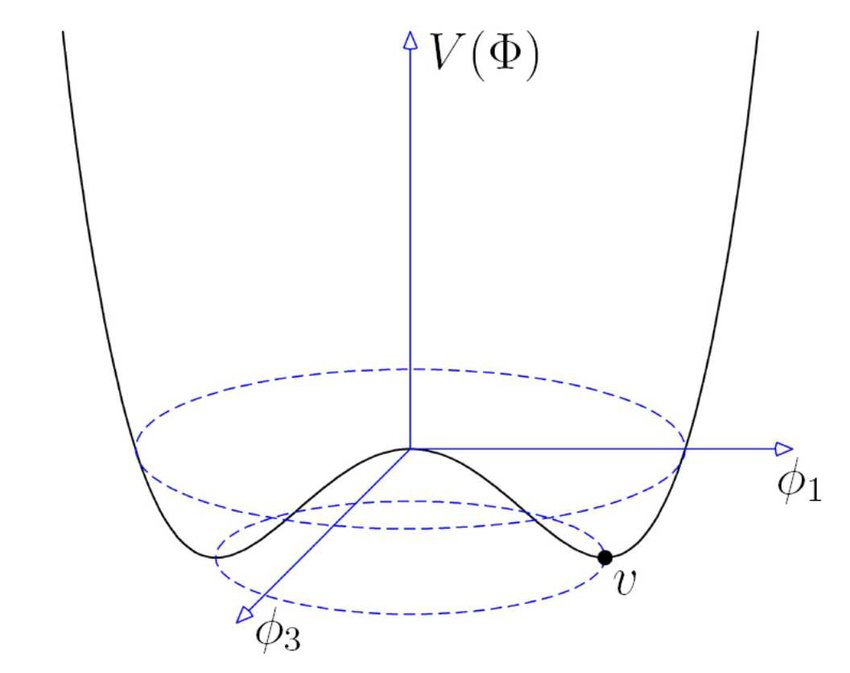
\includegraphics[width=\textwidth]{images/higgs_potential.jpg}
    \caption{Higgs potential, and its typical form. A vacuum solution is highlighted}
    \label{higgs}
\end{figure}
We define the complex components of the fields as follows:
\begin{equation}
    \phi = \phi_1 + i \phi_2
\end{equation}
and we choose the following minimum:
\begin{equation}
    \begin{cases}
        \langle\phi_1\rangle_0 \equiv v = \sqrt{-\dfrac{\mu^2}{\lambda}} \\
        \langle \phi_2\rangle_0 = 0
    \end{cases}
\end{equation}

We define two new fields around the value of the minimum:
\begin{equation}
    \begin{cases}
        \eta = \phi_1 - v\\
        \chi = \phi_2
    \end{cases}
\end{equation}
Substituting the new fields in the Lagrangian we obtain:
\begin{equation}
    \mathcal{L} = \frac{1}{2}(\partial_{\mu}\eta)(\partial^{\mu\eta} + \frac{1}{2}(\partial_{\mu}\chi)(\partial^{\mu}\chi) +\mu^2 \eta^2 
\end{equation}
\begin{equation*}
    - \lambda\left[\frac{1}{4}\left(\eta^2 +\chi^2\right)^2 + v \eta \left(\eta^2 + \chi^2\right)\right] +\text{const.}
\end{equation*}
We can observe that now we obtain two particles, $\eta$ and $\chi$.\\
In particular, $\eta$ is a massive particle with mass:
\begin{equation*}
    m_{\eta} = \sqrt{-2\mu^2}
\end{equation*}
while $\chi$ is massless.\\

We can see that this case is of our interest because it resembles the physical case of the electroweak interaction (a massive particle and a massless one).
However, the complex scalar field theorizes only two particles, while from the experiments we know there are four bosons for this interaction: W$^{\pm}$, Z and the photon.\\This means we have to find a bigger group that can give us 4 bosons. \\
In particular, we need 4 gauge bosons. A specific discussion of spontaneous symmetry breaking in the presence of a gauge symmetry is discussed in the appendix.

\subsection{Non-Abelian case and the Higgs mechanism}
The Higgs mechanism was proposed in 1964 separately by P. Higgs \cite{higgs_art} and R. Brout and F. Englert \cite{brout_art}.\\
We consider the gauge group $SU(2)xU(1)$ \cite{weinberg} and we perform a symmetry break on the global group with the pattern:
\begin{equation}
    SU(2)_L x U(1)_Y \rightarrow U(1)
\end{equation}
We choose to leave a remaining global $U(1)$ symmetry to describe the photon, which stays massless.\\
We take the electroweak Lagrangian from equation \ref{ew_eq}, and we add an additional field, $\Phi$:
\begin{equation}
    \Phi =
    \begin{pmatrix}
        \phi^+\\ \phi_0
    \end{pmatrix}
\end{equation}
This field is what parametrizes the Higgs mechanism. $\phi^+$ is charged while $\phi_0$ is neutral.\\
The complete Lagrangian is:
\begin{equation}
    \mathcal{L}= -\frac{1}{4}A_{\mu\nu}A^{\mu\nu} -\frac{1}{4}B_{\mu\nu}B^{\mu\nu} + \left(D_{\mu}\Phi\right)^{\dagger}\left(D^{\mu}\Phi\right) - V(\Phi^{\dagger}\Phi), 
\end{equation}
where:
\begin{equation}
   \mathcal{L} =  -\frac{1}{4}A_{\mu\nu}A^{\mu\nu}
\end{equation}
is the Yang-Mills Lagrangian for the $SU(2)$ bit, while:
\begin{equation}
    \mathcal{L} = -\frac{1}{4}B_{\mu\nu}B^{\mu\nu}
\end{equation}
takes into account the $U(1)$ part, and:
\begin{equation*}
    V(\Phi^{\dagger}\Phi) = \mu^2(\Phi^{\dagger}\Phi) + \lambda(\Phi^{\dagger}\Phi)^2
\end{equation*}
is the usual quartic potential for the $\Phi$ field, the Higgs field.

We consider $\mu^2<0$ and choose the minimum value of the field to be:
\begin{equation}
    \Phi_{min} = \frac{1}{\sqrt{2}}\begin{pmatrix}
        0 \\ v
    \end{pmatrix}, \quad v \in \mathbb{R}
\end{equation}
As we've already done before, we can parameterize the fluctuations around $\phi_{min}$, and by fixing the gauge as well we find:
\begin{equation}
    \Phi(x) =\frac{1}{\sqrt{2}} \begin{pmatrix}
        0 \\ v + \rho(x)
    \end{pmatrix}
\end{equation}
where $1/\sqrt{2}$ is a conventional normalization.\\

Substituting in the Lagrangian, we can find:
\begin{equation}
    \mathcal{L} = - \frac{1}{4} A_{\mu\nu}A^{\mu\nu} -\frac{1}{4} B_{\mu\nu}B^{\mu\nu} + \frac{1}{2}\partial_{\mu}\rho\partial^{\mu}\rho -V\left(\frac{(v + \rho)^2}{2}\right) +
\end{equation}
\begin{equation*}
    \frac{(v+ \rho)^2}{8}\left[\left(g' B_{\mu} - gA_{\mu}^{(3)}\right) \left(g' B^{\mu} - g A^{(3)\mu}\right) +g^2\left(A_{\mu}^{(1)} A^{(1)\mu} + A_{\mu}^{(2)} A^{(2)\mu}  \right) \right]
\end{equation*}
We can see that we can consider a linear combination of $B_{\mu}$ and the neutral element of the multiplet $A_{\mu}$.\\
That is, we can define new fields:
\begin{equation}
    W_{\mu}^{\pm}= \frac{1}{\sqrt{2}}\left(A_{\mu}^{(1)}\mp A_{\mu}^{(2)}\right), \quad m_W = \frac{vg}{2}
\end{equation}
\begin{equation}
    Z_{\mu} = \frac{1}{\sqrt{g^2 + g'^2}}\left( - g A_{\mu} ^{(3)} + g' B_{\mu} \right), \quad m_Z = \frac{v}{2}\sqrt{g^2 + g'^2}
\end{equation}
\begin{equation}
    A_{\mu} = \frac{1}{\sqrt{g^2 + g'^2}}\left(g A_{\mu} ^{(3)} + g' B_{\mu} \right), \quad m_A = 0
\end{equation}
Requesting the known form for $v$ we can also find the mass of the Higgs boson: $m_H = \sqrt{-2\mu^2}$, as expected from the previous sections, that however depends on a free parameter of the theory, $\mu$.\\
As a side note, we can notice that in this way the mass term for the three fields becomes:
\begin{equation}
    \mathcal{L}_m = \frac{v^2}{4}\left[\left(\frac{g^2 + g'^2}{2}\right)Z_{\mu}Z^{\mu} + g^2 W_{\mu}^{\dagger}W^{\mu}\right]
\end{equation}
So, because of relation \ref{v_relation} the mass term is also proportional to $m_H^2$.
    

\subsection{Fermionic mass terms}

So far, we've seen how the Higgs mechanism allows the gauge boson to have mass (except for the photon, which is massless as expected).\\
We now briefly discuss the mass term for the fermionic side.\\
We define a mass term, called Yukawa interaction, with the form:
\begin{equation}
    \mathcal{L}_m = - G \Phi \Bar{\psi}_R \psi_L,
\end{equation}
where the presence of the doublet of the Higgs field allows the product between the left doublet and the right singlet, and $G$ is an arbitrary constant for each fermion.\\
This is sufficient to describe the leptonic sector, where the Higgs doublet selects only the charged lepton from the doublet (the Higgs mechanism doesn't take into account the mass of neutrinos), but it's not enough for the quarks.\\
Let's consider the mass term separately for up and down quarks:
\begin{equation}
    \mathcal{L}_m = -\left(\Bar{D}_L \Tilde{M}_D D_R + \Bar{U}_L \Tilde{M}_U U_R + \text{h.c.} \right), \quad \Tilde{M}= \frac{v}{\sqrt{2}}Y,
\end{equation}
where we are summing over the three families experimentally observed.\\
The two mass matrices, however, are not diagonal in this form. If we try to diagonalise them simultaneously to obtain the mass eigenstates, we find that it is impossible.\\
We can do it by rotating separately each field, and considering the overall matrix, now diagonal for both the left and right sectors:
\begin{equation}
    \begin{cases}
        U_L \rightarrow V_L^{(U)} U_L\\
        U_R \rightarrow V_R^{(U)} U_R
    \end{cases}
    \hspace{8pt} \Longrightarrow \hspace{8pt}M \equiv V_L^{(U)\dagger}\Tilde{M}V_R^{(U)} \hspace{12pt} \text{diagonal}
\end{equation}
and applying the same procedure on the down sector.\\
However, the newly defined fields introduce a new term in the charged current of the weak interaction:
\begin{equation}
    \mathcal{L}_{CC} = - \frac{g}{\sqrt{2}}\Bar{U}_L\gamma^{\mu}V_L^{(U)\dagger}V_L^{(D)}D_L + h.c. \equiv - \frac{g}{\sqrt{2}}\Bar{U}_L\gamma^{\mu}V_{CKM}D_L + h.c.
\end{equation}
The $V_{CKM}$ describes the mixing between up and down flavours, and introduces the CP violation in the weak sector. It is described by four independent parameters, 3 angles and a phase.\\

We can now write the complete Lagrangian for the SM:
\begin{equation}
    \mathcal{L} = -\frac{1}{4}F_{\mu\nu}F^{\mu\nu} + i\bar{\psi}\slashed{D}\psi +\text{h.c.} + \psi_i Y_{ij}\psi_j \Phi  +\text{h.c.} + |D_{\mu}\Phi|^2 -V(\Phi)
\end{equation}
We also report the characteristics of the SM particles in appendix \ref{app_particles}.

\section{Physics of the Higgs boson and recent results}
The Higgs boson was experimentally observed in 2012 at LHC simultaneously by the experiments CMS and ATLAS.\\
The most precise measurement of its mass by the CMS experiment \cite{art_nature_cms} is:
\begin{equation}
    m_H = 125.38 \pm 0.14 \text{GeV} 
\end{equation}
It is a scalar boson that has non-zero coupling with all fermions and with the weak bosons.
This means that there are multiple production modes, and multiple decay channels.\\
The magnitude of the coupling is deeply related to the particle's mass because, as we pointed out in the previous paragraphs, the coupling of the Higgs boson goes with $m_H^2$ for gauge bosons, and $m_H$ for fermions.
\subsection{Production modes}
The most common production modes in a hadronic accelerator as LHC  are the following: gluon-gluon fusion (ggH), vector boson fusion (VBF), vector-boson associated production (VH) and top pair associated production (ttH).\\
More in detail:
\begin{itemize}
    \item gluon-gluon fusion (ggF) is the predominant production mode, which accounts for approximately 85\% of the total cross-section. The interaction of the gluons with the Higgs boson is performed via quantum loops, as illustrated in fig. \ref{ggf_feynman}, where the predominant contribution is given by diagrams where the loop is made of top and, in lesser measure, bottom quarks;
    \item vector-boson fusion (VBF) is the second mode of production for relevance after ggH, and accounts for approximately 7\% of the total cross-section. The leading diagram, illustrated in fig.,  has two quarks, coming from the proton scattering, interact in the t or u channel, exchanging two vector bosons, which then interact as well through the s channel, emitting a Higgs boson. Because of the low transverse momentum exchange in comparison to the center of mass energy of the two interacting quarks, the signature of this mode of production is the presence of two jets with high rapidity. Furthermore, because this mode doesn't have diagrams that involve QCD, it has higher sensitivity in comparison to ggH;
    \item vector-boson associated production (VH) has an even lower production rate, accounting for 4\% of the total cross-section, and its main diagram has the radiation of a Higgs boson from a vector boson, as illustrated in fig. The signature of this mode is the presence of additional leptons (specifically $e$ and $\mu$) in the leptonic decay of the vector bosons involved;
    \item top pair associated production (ttH) is the mode with the least production rate among the ones listed, with a contribution of about 1\% over the total cross-section. However, it's interesting because its signature is consistent, having two quark top, which almost exclusively decay in Wb, and the decay products of these particles.
\end{itemize}


\begin{figure}[h]
    \centering
    \begin{subfigure}{0.55\textwidth}
    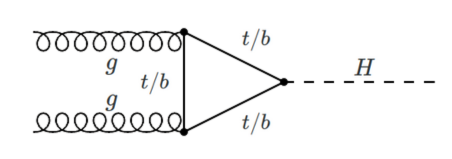
\includegraphics[width=\textwidth]{images/ggh.png}
    \caption{ggH production mode}
    \label{ggf_feynman}
    \end{subfigure}
    \hfill
    \begin{subfigure}{0.3\textwidth}
    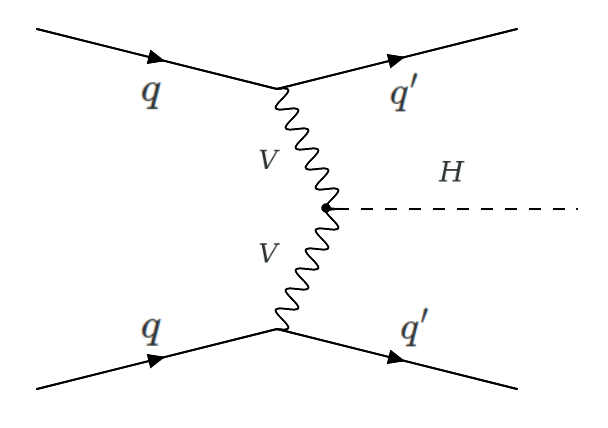
\includegraphics[width=\textwidth]{images/vbf.png}
    \caption{VBF production mode}
    \label{vbf_feynman}
    \end{subfigure}\vspace{5pt}
    \begin{subfigure}{0.55\textwidth}
    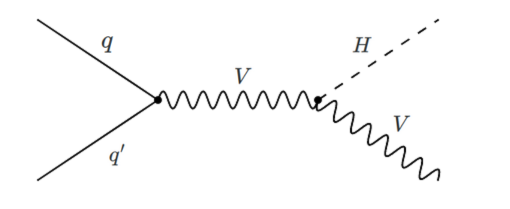
\includegraphics[width=\textwidth]{images/vh.png}
    \caption{VH production mode}
    \label{vh_feynman}
    \end{subfigure}\hfill
    \begin{subfigure}{0.3\textwidth}
    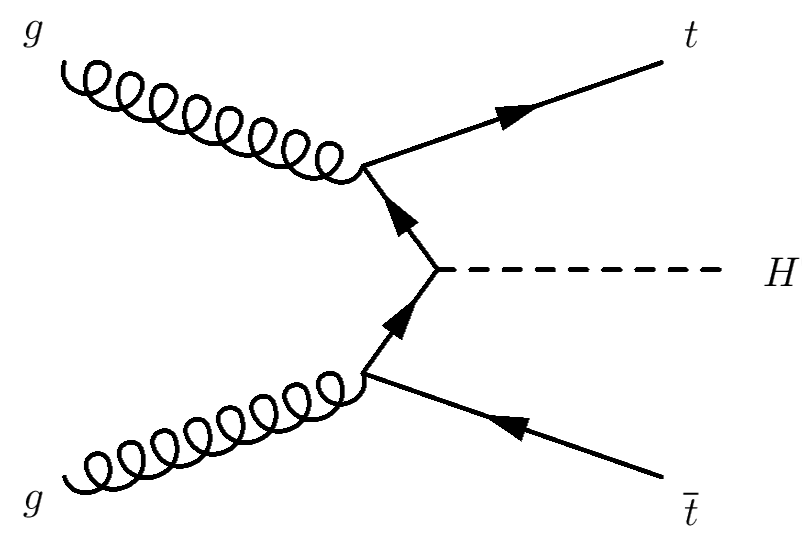
\includegraphics[width=\textwidth]{images/tth.png}
    \caption{ttH production mode}
    \label{tth_feynman}
    \end{subfigure}

    \caption{Feynman diagrams for leading production modes}
    \label{prod_feynman}
\end{figure}
A comprehensive plot of the theoretical cross-sections is presented in fig \ref{cross-section}, along with the pair production cross-section.

\begin{figure}
    \centering
    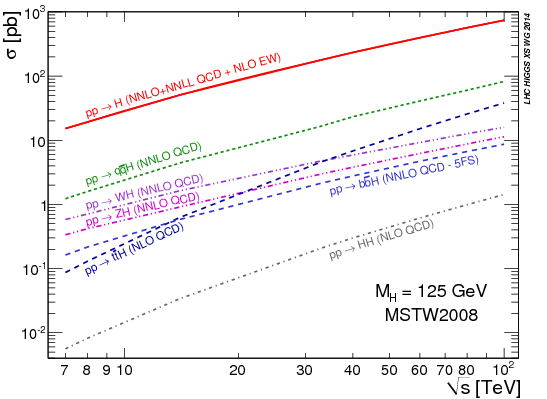
\includegraphics[width= \textwidth]{images/cross_section.png}
    \caption{Plot for the cross-sections as a function of CM energy}
    \label{cross-section}
\end{figure}
Table reports the theoretical cross-section divided by mode.
\begin{table}[ht]
    \centering
    \begin{tabular}{c|c}
         Process & Cross-section [pb]\footnotemark \\\hline
         ggF &  $48.6^{+2.7}_{-3.6}$ \\\hline
         VBF  & $3.78 \pm 0.08$\\\hline
         WH & $1.67\pm 0.03$\\\hline
         ZH & $0.88^{+0.04}_{-0.03}$ \\\hline
         t$\Bar{\text{t}}$H & $0.50^{+0.03}_{-0.04}$\\\hline 
    \end{tabular}
    \caption{Theoretical cross-sections for the predominant production modes for a Higgs boson of m$_H$ = 125 GeV and $\sqrt{s}$ = 13 TeV}
    \label{tab:cross-section}
\end{table}
\footnotetext{the unit of measure for cross-sections is the barn, which corresponds to $10^{-24} \text{cm}^2$. Usually, cross-section are in the order of pb ($10^{-12}$b) or fb ($10^{-15}$b)}
\subsection{Decay channels}
Because the Higgs boson is an unstable particle, it decays.\\
Its SM theoretical width is \cite{higgs_width}:
\begin{equation}
    \Gamma_H = 4.14 \pm 0.02 MeV \Longrightarrow \tau_H = \frac{\hbar}{\Gamma_H} \approx 1.6 \cdot 10^{-22} s
\end{equation}
Because of the small lifetime, the only way to detect the Higgs boson is through is decay products.\\ 
As already stated, the coupling of the Higgs boson is proportional to the mass of the particles (or the squared mass in the case of boson vectors), so the favoured channels are the ones with the gauge bosons and the third generation of fermions, that is, b quark and tau lepton, because the top quark is too heavy.\\
A comprehensive plot of the decay channels is presented in fig. \ref{higgs_br}, while table \ref{BR_teor} contains the theoretical branching ratios for the principal decay channels.\\
\begin{figure}[ht]
    \centering
    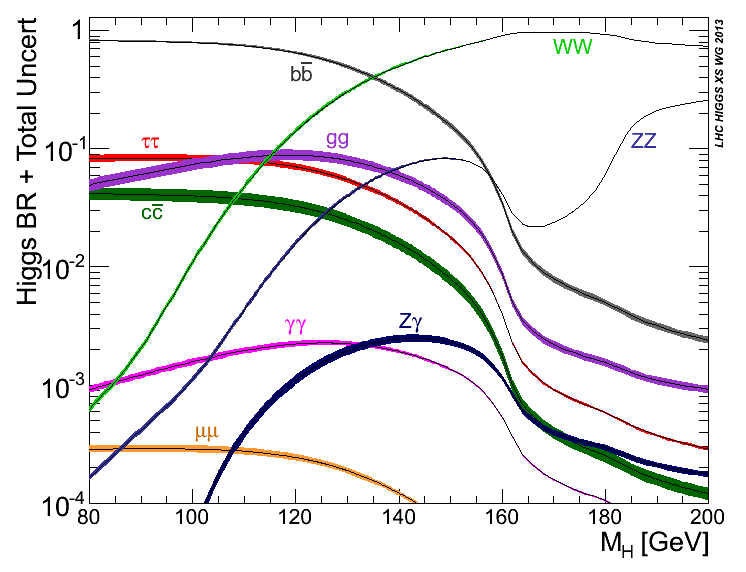
\includegraphics[width = \textwidth]{images/br.png}
    \caption{Branching ratios of the Higgs boson decay as a function of the mass}
    \label{higgs_br}
\end{figure}
\begin{table}[ht]
    \centering
    \begin{tabular}{c|c}
        Decay channel & Branching ratio [\%] \\\hline
        H $\rightarrow b\Bar{b} $ & 58.2\\  \hline
        H $\rightarrow$ $W^+ W^-$ & 21.4 \\\hline
        H $\rightarrow \tau^+ \tau^-$ & 6.27 \\\hline 
        H $\rightarrow$ ZZ & 2.6 \\\hline
        H $\rightarrow$ $\gamma\gamma$ & 0.22 \\\hline
        H $\rightarrow$ ZZ $\rightarrow$ $\mu, e$ & 0.03 \\\hline

    \end{tabular}
    \caption{Theoretical values for the branching fractions of the Higgs decay. The channel where the two Z from the Higgs decay go into charged leptons is called "\textit{golden channel}", because it provides a very high sensitivity}
    \label{BR_teor}
\end{table}
It should be noted that because the Higgs doesn't directly interact with the photon, the branching ratio $H\rightarrow\gamma\gamma$ provides us further information about the coupling of the particle inside the loop, which in this case can be either bosonic or fermionic, as it can be seen from fig. \ref{gamma_coupling}
\begin{figure}[ht]
    \centering
    \begin{subfigure}{0.4\textwidth}
        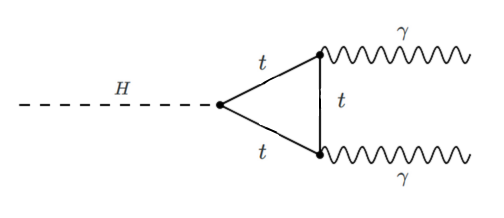
\includegraphics[width=\textwidth]{images/gamma_top.png}
        \caption{Fermionic loop}
        \label{gamma_top}
        \end{subfigure}
    \begin{subfigure}{0.4\textwidth}
        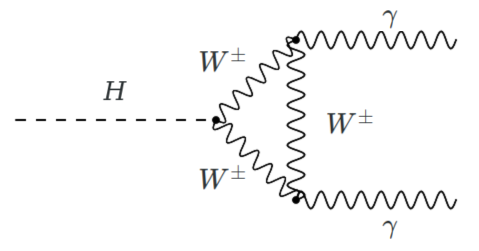
\includegraphics[width=\textwidth]{images/gammaW.png}
        \caption{Bosonic loop}
        \label{gamma_W}
        \end{subfigure}
    \caption{Feynman diagrams for the quantum loops that give the coupling of the Higgs boson with $\gamma$. In \ref{gamma_top} only the main contribution for the top is shown, while for \ref{gamma_W}, electrically charged bosons are the only boson admitted because of the coupling with the photon}
    \label{gamma_coupling}
\end{figure}
\subsection{Known issues}
Despite solving the mass problem for both the fermionic and bosonic sectors, the formulation of the SM still has some criticalities that can't be resolved with the current theory. \\
Assuming the absence of new physics, issues like the flavour puzzle, the neutrino masses don't find an explanation.\\
Assuming BSM physics instead, solutions for the aforementioned problems can be found, leading however to other criticalities. %Possible solutions proposed through the years are the Supersymmetry (SUSY) and the Composite Higgs.
\subsubsection{Hierarchy problem}
%It is a direct consequence of assuming new BSM physics, particularly considering SM as a low-energy limit. \\
%In this approach, SM is considered non-renormalizable. This means, in general, that no terms are cancelling each other to obtain finite quantities.\\
For the Higgs boson, the radiative corrections to the mass are much larger than the mass itself. Assuming no intermediate energy scale between SM and the Planck scale (which is the natural cutoff scale), the radiative correction given from the new physics contribution would be:
\begin{equation}
    \Delta m_H^2 \sim \frac{1}{16 \pi^2}M_P^2 \simeq 10^{36} \text{  GeV}^2, 
\end{equation}
where $M_P$ is the Planck mass.\\
\begin{figure}[ht]
    \centering
    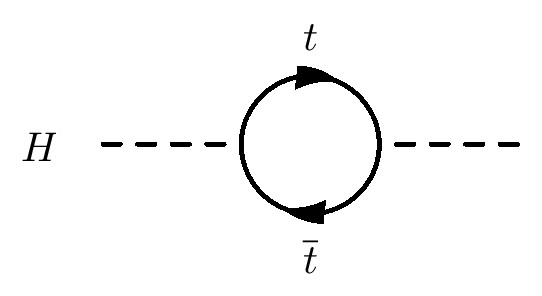
\includegraphics[width= 0.5\linewidth]{images/radiative_corrections_H.png}
    \caption{Leading Feynman diagram for the Higgs radiative corrections; in this case, a quark top and its antiparticle run in the loop. This diagram in particular gives a contribution proportional to the squared value of the considered scale energy}
    \label{radiative_correction}
\end{figure}
To obtain the experimental value, a subtle process of fine-tuning would be needed, so delicate that most of the theorists find it unnatural.\\
A solution would be to consider an intermediate energy scale, around the TeV, that would lead to a more reasonable tuning.
\subsection{Theoretical solutions}
Several solutions have been proposed to solve the known problems of the SM. We report two of the most relevant.\\
\subsubsection{Supersymmetry}
Supersymmetry (SUSY) \cite{susy} is a framework proposed around the 1970s by several physicists independently and that aims to extend the SM.\\
It focuses on the idea that, because of the radiative corrections, the mass of the boson itself should be extremely large. However, this prediction doesn't correspond to the experimental observations made at LHC. \\
SUSY theories predict the existence of several new particles that would help cancel out the contributions to the Higgs mass from the SM particles, allowing the existence of a light Higgs boson. These extra particles are partners of the SM ones, and in particular, would act as a link between the fermions and the bosons, in the sense that a fermionic SM particle would have a bosonic SUSY partner, and vice versa.\\
Because of the internal symmetries of SUSY, the lightest of the newly introduced particles should have a mass of around 100 GeV, and should be stable.\\
However, to date, no relevant experimental indication of the existence of SUSY particles has been observed. \\
LHC, its upgrade HL-LHC and future colliders are expected to further test this framework.\\
\subsubsection{Composite Higgs Models}
Composite Higgs Models (CHM) \cite{chm} consider an alternative approach that assumes the Higgs boson not to be an elementary particle, but a composite state of some new particles. \\
In the models where the Higgs is a Goldstone boson coming from spontaneous symmetry breaking, a larger group of symmetry is considered, which contains the $SU(2)x U(1)$ group of the SM.\\
The larger group then breaks into the SM group that we know, creating a set of (pseudo)Nambu-Goldstone bosons, among which the Higgs boson is included.\\
In CHM, the quadratic divergences from the radiative corrections are solved with the physical cutoff of the compositness scale.\\
To keep a reasonable tuning to the SM, the new energy scale should remain around the TeV scale.\\
LHC, its upgrade HL-LHC and future colliders will be able to test CHM indirectly and directly.

%\section{Why study the self-coupling of the Higgs boson}
\section{Higgs pair production and self-coupling}
In the previous sections, we've discussed the contributions of the Higgs field in the justification of a mass term for the different elementary particles described by the SM.\\
However, we've never explicitly written the complete potential.
And that is because the actual shape of the Higgs potential is unknown.\\
We can rewrite the potential as:
\begin{equation}
    V(\rho(x)) = \frac{1}{2}m_H^2\rho(x)^2 +\lambda v \rho(x)^3 + \frac{1}{4}\lambda\rho(x)^4 +\text{const}
\end{equation}
by expanding the quartic potential and substituting the expansion of the field around the minimum $v$.\\
So, by studying the triple and quartic coupling of the Higgs boson we can study directly the shape of the scalar potential by studying the value of $\lambda$.\\
From the definition of $v$ we can find an explicit form for $\lambda$:
\begin{equation}
    v^2 = -\dfrac{\mu^2}{\lambda} \Longrightarrow \lambda = -\dfrac{\mu^2}{v^2} = \dfrac{m_H^2}{2v^2} 
\end{equation}
Both $m_H$ and $v$ are values observed experimentally, the first by direct measurement, the second by studying the mass of the W and Z bosons, so we have a rough estimate of it:
\begin{equation}
    \lambda \approx 0.13
\end{equation}
The theoretical cross-section for the pair production is, considering only ggF as production mode and with $\sqrt{s}$ = 13 TeV \cite{theoretical_pair_prod}:
\begin{equation}
    \sigma(gg\longrightarrow H H )_{ggF} = 31.31 \text{fb}^{+0.66\%}_{-2.8\%}
\end{equation}
The dominant Feynman diagrams are shown in fig. \ref{pair_prod}. \\
It can be seen that di-Higgs events can be produced via a box diagram, where heavy fermions run (in particular t and b quarks), and via the Higgs boson self-coupling.\\
We can write the interaction Lagrangian as:
\begin{equation}
    - \mathcal{L} =\left(\frac{m_H^2}{2 v} \right)\lambda_{HHH} H^3 + \frac{m_t}{v} \Bar{t}g_t t H,
    \end{equation}
where the first term describes the self-coupling diagram, and the second term describes the box diagram.\\
The two processes interfere destructively, and the cross-section is minimum near the SM value, as can be seen from fig. \ref{cms_coupling}.
This means that a small increase in the value of $\lambda_{HHH}$ decreases the expected HH production cross-section, and so modifies the distributions of event kinematics.
\begin{figure}
    \centering
    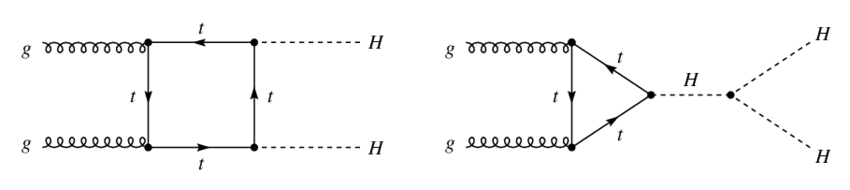
\includegraphics[width= 0.8\linewidth]{images/pair_production.png}
    \caption{Dominant Feynman diagrams for the Higgs pair production. On the left, the box diagram; on the right, the Higgs boson self-coupling-}
    \label{pair_prod}
\end{figure}
    \begin{figure}
    \centering
        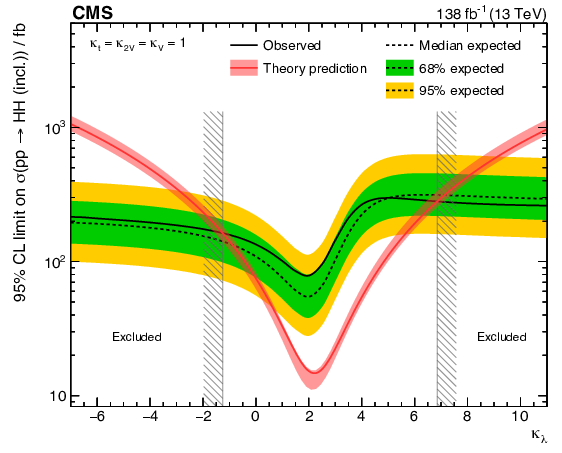
\includegraphics[width=0.8\textwidth]{images/selfcoupling_cms_HH.png}
        \caption{Limits on the Higgs boson self-interaction set from the CMS experiment}
        \label{cms_coupling}    
\end{figure}
To study the self-coupling, the two modes need to be distinguished.\\
It should be noted that because the self-coupling diagram contains a propagator in the s-channel, its relevance should decrease at higher energies because of its behaviour like $1/s$ for energies at the centre of mass considerably higher than $m_H$. Therefore, the box diagram gives on average more energetic Higgs boson pairs than the triangle diagram, so the opening angle between the decay products of each boson can be useful to isolate the self-coupling diagram \cite{theo_pair}.\\
There is also an alternative approach to studying the self-coupling of the Higgs boson, and that is to measure deviations of the inclusive and differential single H production rates \cite{HL-LHC_Higgs}. The contributions of the self-coupling in the single H production can be mainly found in the production in association with top quarks ($t\Bar{t}H$) or single-top production (tH), because of the large mass of the top quark, and consequently, the large coupling with the Higgs boson.\\
A study of the differential production cross-section as a function of the distribution of $p_T^H$ can be done, for example, considering $\gamma\gamma$ as a final state for the possibility of having a fully reconstructed event, and from which the effects of a modified H boson self-coupling can be extrapolated.\\
This gives an ulterior mode to test the physics of the SM Higgs boson, complementary to the direct search of Higgs pair production.
%\subsection{Possible implications of the HH measurements}
%A brief summary of possible results closely related to the Higgs pair production are listed.
%\subsubsection{Electroweak phase transition}
%One of the open problems of high energy physics and cosmology is the origin of matter-antimatter asymmetry. One of the solutions proposed is the electroweak baryogenesis, where the asymmetry is tied to the electroweak symmetry breaking. In this scenario, the universe is supposed to have gone from electroweak symmetric to broken phase at a temperature T$_{EW} \sim 100$ GeV. If such a transition occurred, there must have been some CP-violating interactions that were active in those instants and that justify the now observed asymmetry. However, the current formulation of the SM doesn't meet any of these two requirements: the symmetry breaking given from a 125 GeV Higgs boson doesn't cause the phase transition, and the CP violation from the $V_{CKM}$ isn't enough to justify the observed asymmetry. For this reason, viable electroweak baryogenesis needs BSM physics that couples with the Higgs boson.\\
%Deviation from the SM pair production cross-section and anomalous self-coupling can be a viable way to indirectly probe the existence of new interactions needed for the electroweak phase transition to occur even with a 125 GeV Higgs boson.
%\subsubsection{Vacuum stability}

\subsection{Results on the measurement}
\subsubsection{CMS}
The following results were published in 2022. In plot \ref{cms_results} we show the ratio between the observed cross-section and the SM one for Higgs pair production, divided per year and per final state (and their combination). \\
\begin{figure}[ht]
    \centering
        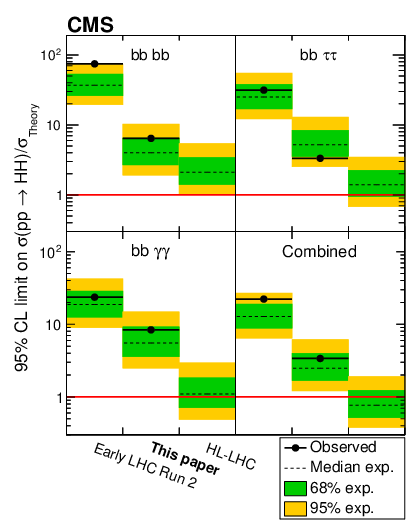
\includegraphics[width=0.7\textwidth]{images/cms_expected_HH_time.png}
        \caption{Recent results and projections from the CMS experiment on the production of Higgs pairs}
    \label{cms_results}  
\end{figure}
A 95\% confidence level observed (expected) upper limit on the combined non-resonant production cross-section is set at \cite{res_CMS_combined}:
\begin{equation}
    \sigma_{obs} \left(\sigma_{exp}\right) = 3.4 (2.5)\text{  }\sigma_{SM}
\end{equation}
\subsubsection{ATLAS}
The following results were published in 2023\cite{atlas_combined}. In plot \ref{atlas_results} we show the cross-section measured in the various decay channels (and their combination)\\
A 95\% confidence level observed (expected) upper limit on the combined non-resonant production cross-section is set at:
\begin{equation}
        \sigma_{obs} \left(\sigma_{exp}\right) = 2.4 (2.9)\text{  }\sigma_{SM}
\end{equation}
on the double-Higgs signal strength, defined as the sum of the ggF HH and VBF HH production cross-sections normalised to its SM prediction
\begin{figure}[ht]
    \centering
        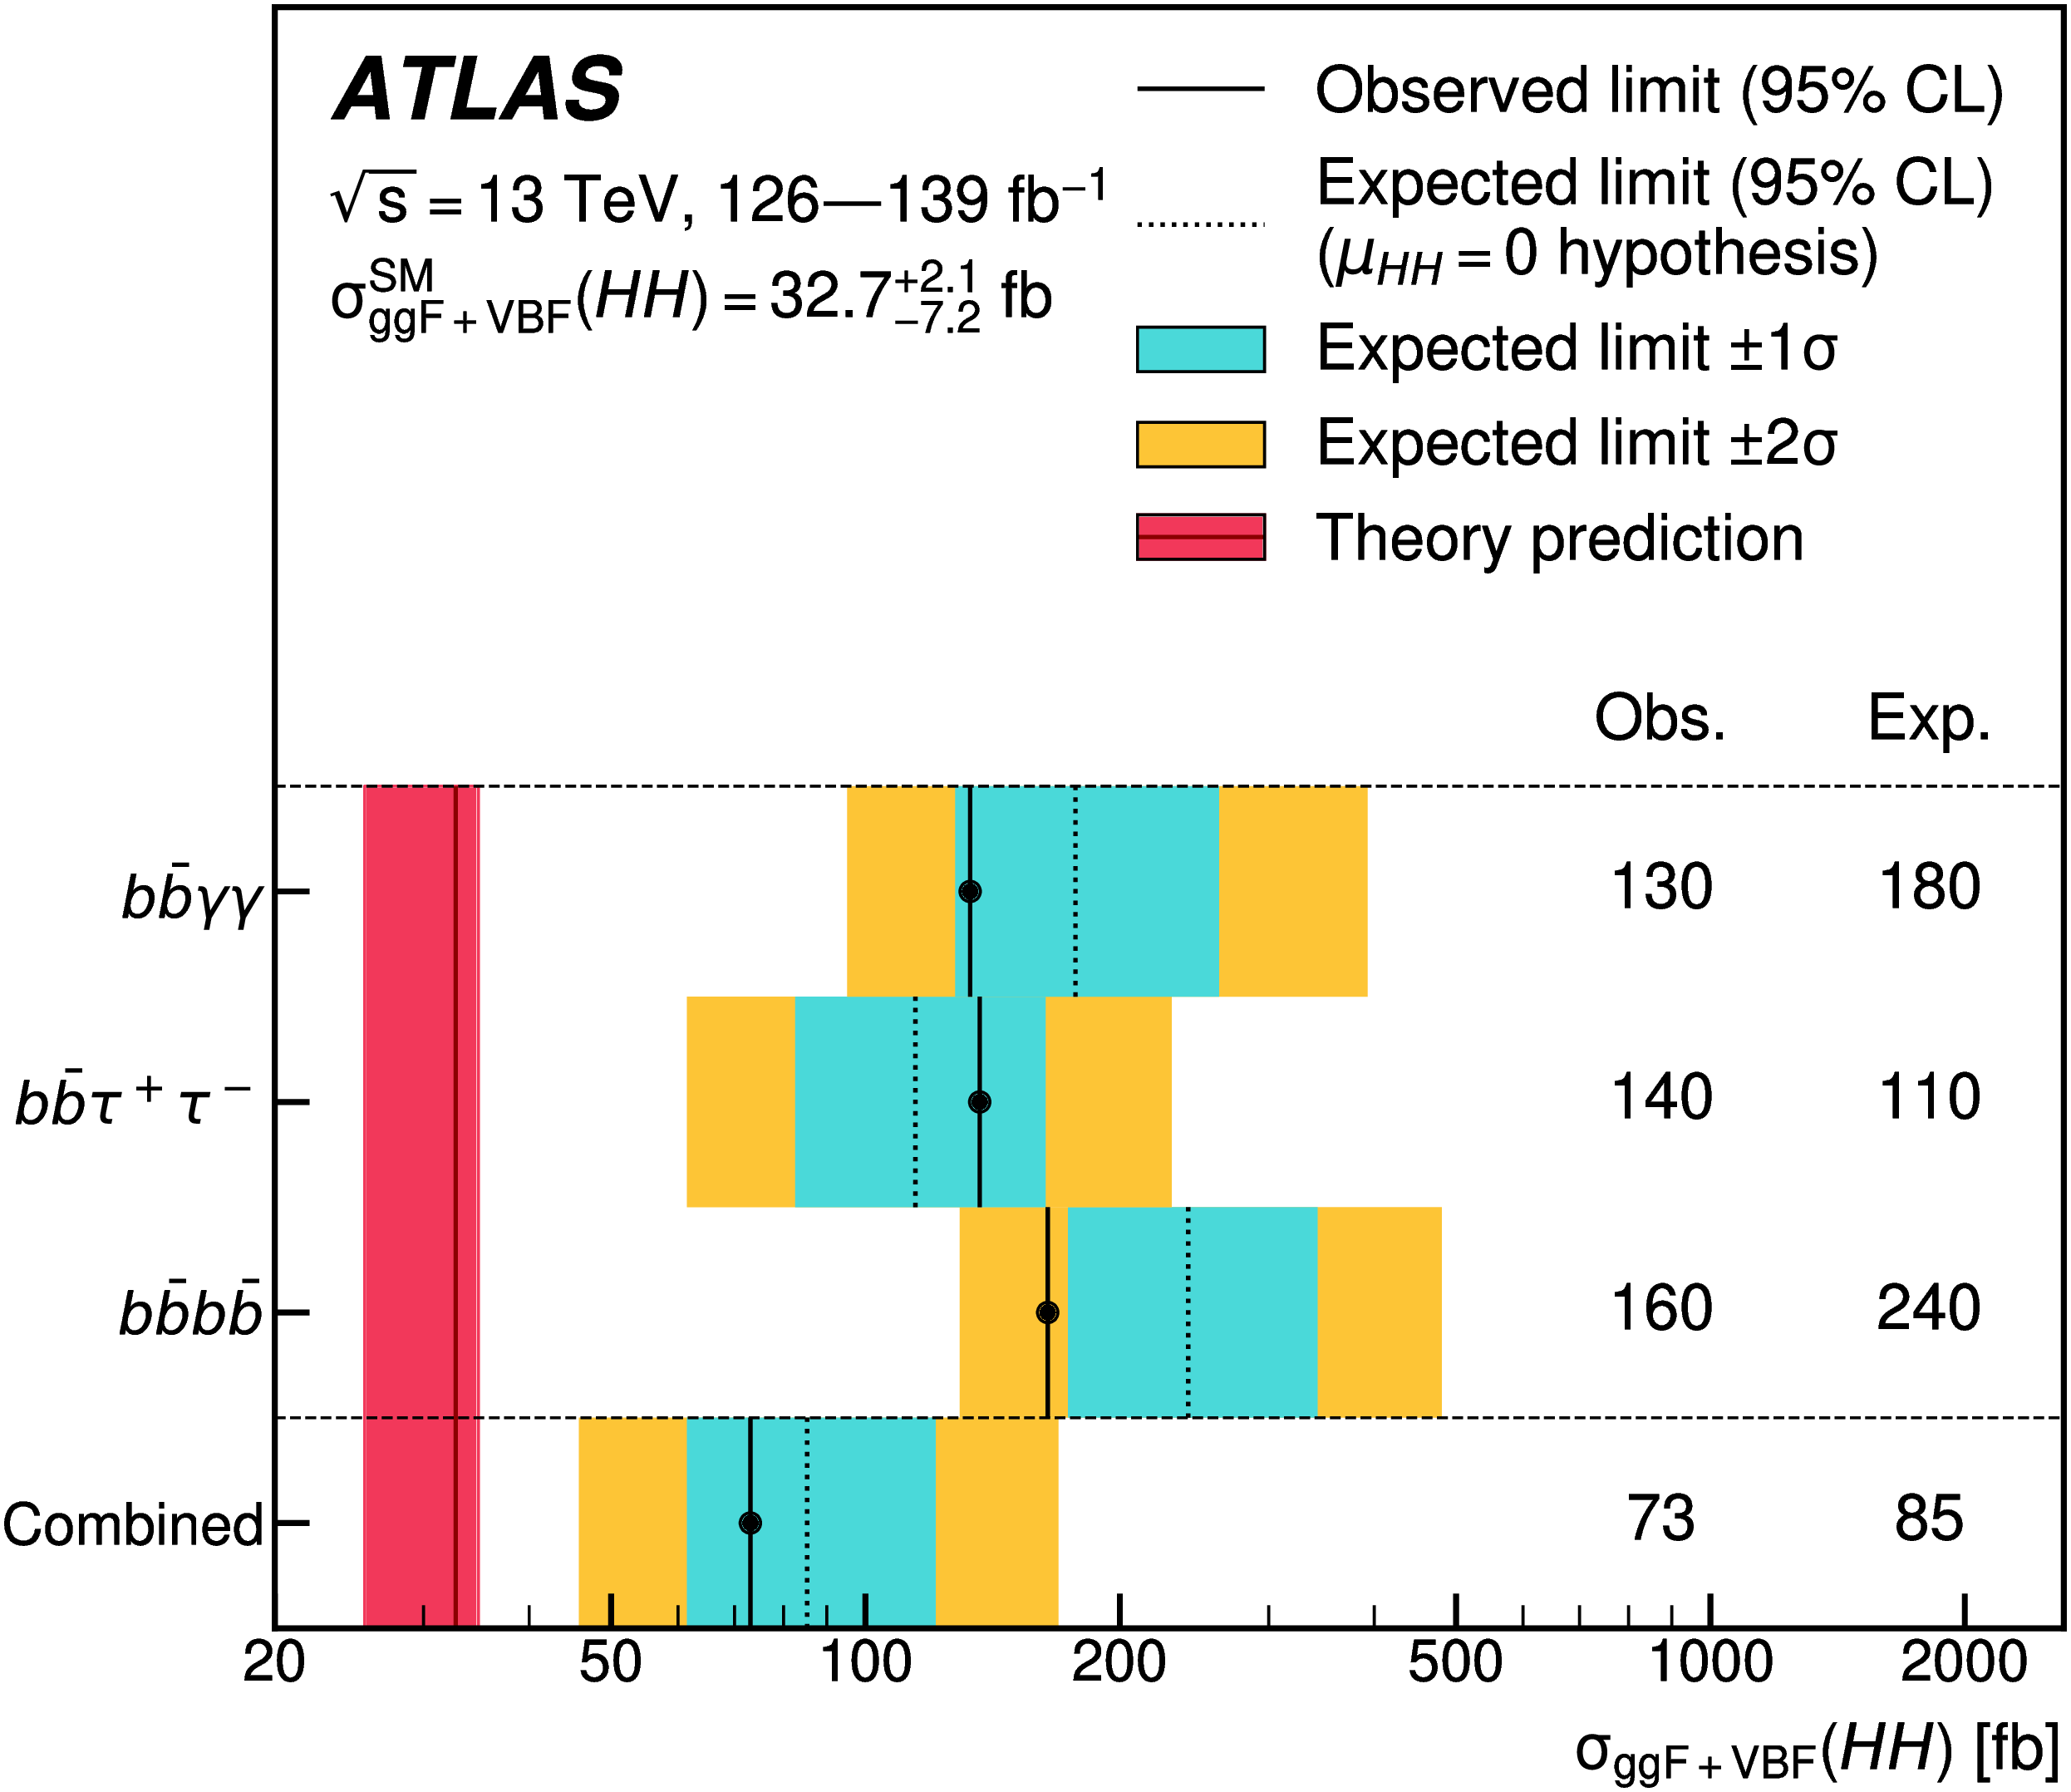
\includegraphics[width=0.7\textwidth]{images/atlas_expected.png}   
    \caption{Limits on the production of Higgs boson pairs set by the experiment ATLAS}
    \label{atlas_results}  
\end{figure}
\chapter{LHC and the CMS experiment}
\label{chap:chapter_3}
A brief introduction to the collider LHC \ref{sec:lhc} and the experiment CMS \ref{sec:cms} is provided, along with technical information. In section \ref{sec:HL-LHC} the High-Luminosity LHC upgrade is discussed, with a particular focus on its physics program and the study of the Higgs self-coupling.

\section{LHC}
\label{sec:lhc}
The Large Hadron Collider (LHC) is the largest and most powerful particle collider constructed so far, located near Geneva, Switzerland, and built by the European Organization for Nuclear Research (CERN).  

The LHC is located underground, and it uses the tunnel of a previous collider, the Large Electron-Positron Collider (LEP), a ring of about 27 km in circumference and situated over 100 metres underground.

The LEP was active from 1989 to 2000 and collided electrons and positrons with centre of mass energy of $\sqrt{s} = 91$ GeV up to 200 GeV in the later stages of the project.  

Notable results obtained from LEP are the discovery of Z and $W^{\pm}$ bosons, and the estimation of the number of light neutrinos.

The LHC started its collision in 2010, and it was constructed to probe the physics of the SM and beyond, in particular to search for the Higgs boson, discovered in 2012.

It relies on a complex structure of accelerators to provide beams of protons currently colliding at centre of mass energy of $\sqrt{s} = 13.6$ TeV.

\subsubsection{Technical characteristics}

The main idea around which revolves LHC (and previously LEP) is the concept of the synchrotron, an accelerating technique in which the accelerated particles travel around a fixed circular path.\\
To obtain this, the magnetic field that bends the trajectory is increased with time to keep it synchronized with them, hence the name.\\
Obviously, because of the very high energies provided to the particles (6.5 TeV per proton), one synchrotron is not enough, and that is why CERN is a complex structure of accelerators and storage rings, as can be seen in fig. \ref{cern_complex}.
\begin{figure}
    \centering\includegraphics[width=\textwidth]{images/CERN_accelerator_complex.jpg}
    \caption{CERN accelerator complex, with the position of the various experiments highlighted as well}
    \label{cern_complex}
\end{figure}

Discussing specifically the LHC collider, as already stated, it consists of an underground tunnel of 26.7 km. The choice of an underground facility was made for economical convenience, and also to have the natural shielding of the Earth's crust against background radiation.\\
The tunnel contains two beam pipes in which the particles travel in opposite directions, and which intersect at four different points, where the four main experiments are located, allowing the particle collisions. The trajectory of the particles is ensured by 1232 dipole magnets, and an additional 392 quadrupole magnets are used to keep the beams focused, with particular attention around the interaction points.\\ 
All the magnets, made of copper-clad niobium-titanium, are superconducting magnets, and operate at the temperature of 1.9 K (-271.25 $^{\circ}$C), which is provided with the use of superfluid helium-4. In this way, a magnetic field of up to 8.3 T is obtained.\\
To have better control over the acceleration and collisions, the beams are not continuous, rather the protons are bunched together in bunches long about 8 cm. In this way, collisions happen every 25 ns, and this leads to a bunch collision rate of 40 MHz.\\
The bunches are accelerated using radiofrequency cavities, where the electromagnetic field oscillates at a tuned frequency, delivering energy to the protons.
Radiofrequency cavities are also extremely useful in keeping the bunches compact because, when the beam has reached its maximum energy, an ideally timed proton won't be further accelerated, while, if the timing of the proton is slightly different from the tuning, it will be accelerated (delayed) or decelerated (anticipated), guaranteeing the desired energy to each proton and the keeping of the bunch structure.  
\subsubsection{Luminosity}
The luminosity is defined as the ratio between the rate of events of a considered process and the cross-section of that process:
\begin{equation}
    L = \frac{R}{\sigma} \quad [cm^{-2}s^{-1}]
\end{equation}
In the specific case of a circular accelerator, with the assumption of Gaussian profiles in all dimensions, and assuming equal beams in both directions, we can define the instantaneous luminosity as:
\begin{equation}
    L = \dfrac{N_1N_2N_b f}{4\pi\sigma_x\sigma_y},
    \label{luminosity}
\end{equation}
where $N_1 \text{and} N_2$ are the particles in the two beams, $N_b$ is the number of bunches, $f$ is the frequency of interaction, and $\sigma_x \text{and} \sigma_y$ are the bunch lengths over the two directions.\\
The average peak luminosity provided from LHC during the Run2 has been of $L =  2.1 \cdot 10^{34} cm^{-2}s^{-1}$, doubling the value from Run1, of {}.\\ 
However, this level of luminosity brings a disadvantage, that is, the presence of pile-up collisions. \\
Pile-up collisions indicate the number of additional proton-proton collisions that happen in the same bunch, and that generate background noise. To make an example, during Run2, the average pile-up collisions amounted to  
Integrating \ref{luminosity} over time, we find the integrated luminosity, which is the total number of collisions produced over a period of time.\\
A plot of the integrated luminosity over time and up to 2018 is reported in plot \ref{luminosity}
\begin{figure}
    \centering
    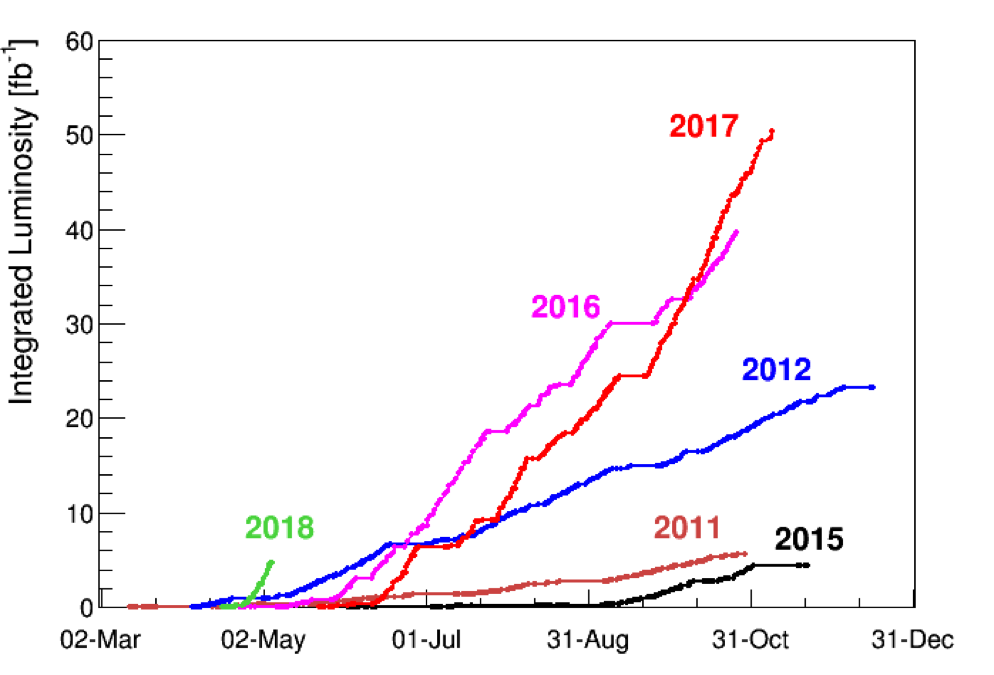
\includegraphics[width= \textwidth]{images/luminosity.png}
    \caption{Integrated luminosity over time}
    \label{luminosity}
\end{figure}
Integrated luminosity is a crucial parameter to take into account because most of the studied processes are rare, and statistics is needed.\\
\subsubsection{Reference frame}
We consider a right-handed coordinate system, where the z axis is parallel to the beam direction.\\
We then define the azimuthal angle $\phi$ as the angle in the xy plane, and the polar angle $\theta$ in the z direction.\\
The typical kinematic variables for the particles are:
\begin{itemize}
    \item $p_T$: the transverse momentum, defined as the amount of momentum perpendicular to the beam direction;
    \item $\phi$;
    \item $m$: the invariant mass of the particle;
    \item $\eta$: the pseudorapidity, defined as 
    \begin{equation*}
        \eta = \frac{1}{2}\ln(\frac{|p|+ p_z}{|p| - p_z}) = - \ln(\tan\frac{\theta}{2})
    \end{equation*}
    is another way to indicate the angle of the particle with the z axis; it is 0 if the particle is perpendicular to the beam direction, and it's greater the more the particle is aligned to the beam direction.
\end{itemize}
\section{CMS}
\label{sec:cms}
The Compact Muon Solenoid (CMS) is one of the main experiments at LHC. It's a general-purpose experiment, that is, it was designed to be able to observe any phenomena the LHC might reveal.\\
It is 15 metres high and 21 metres long, and it weighs 14000 tons.\\
A schematic summary of the overall structure of the detector is reported in fig. \ref{cms}.\\
Further reading on the original project can be found at Ref. \cite{cms_detector}
\begin{figure}
    \centering
    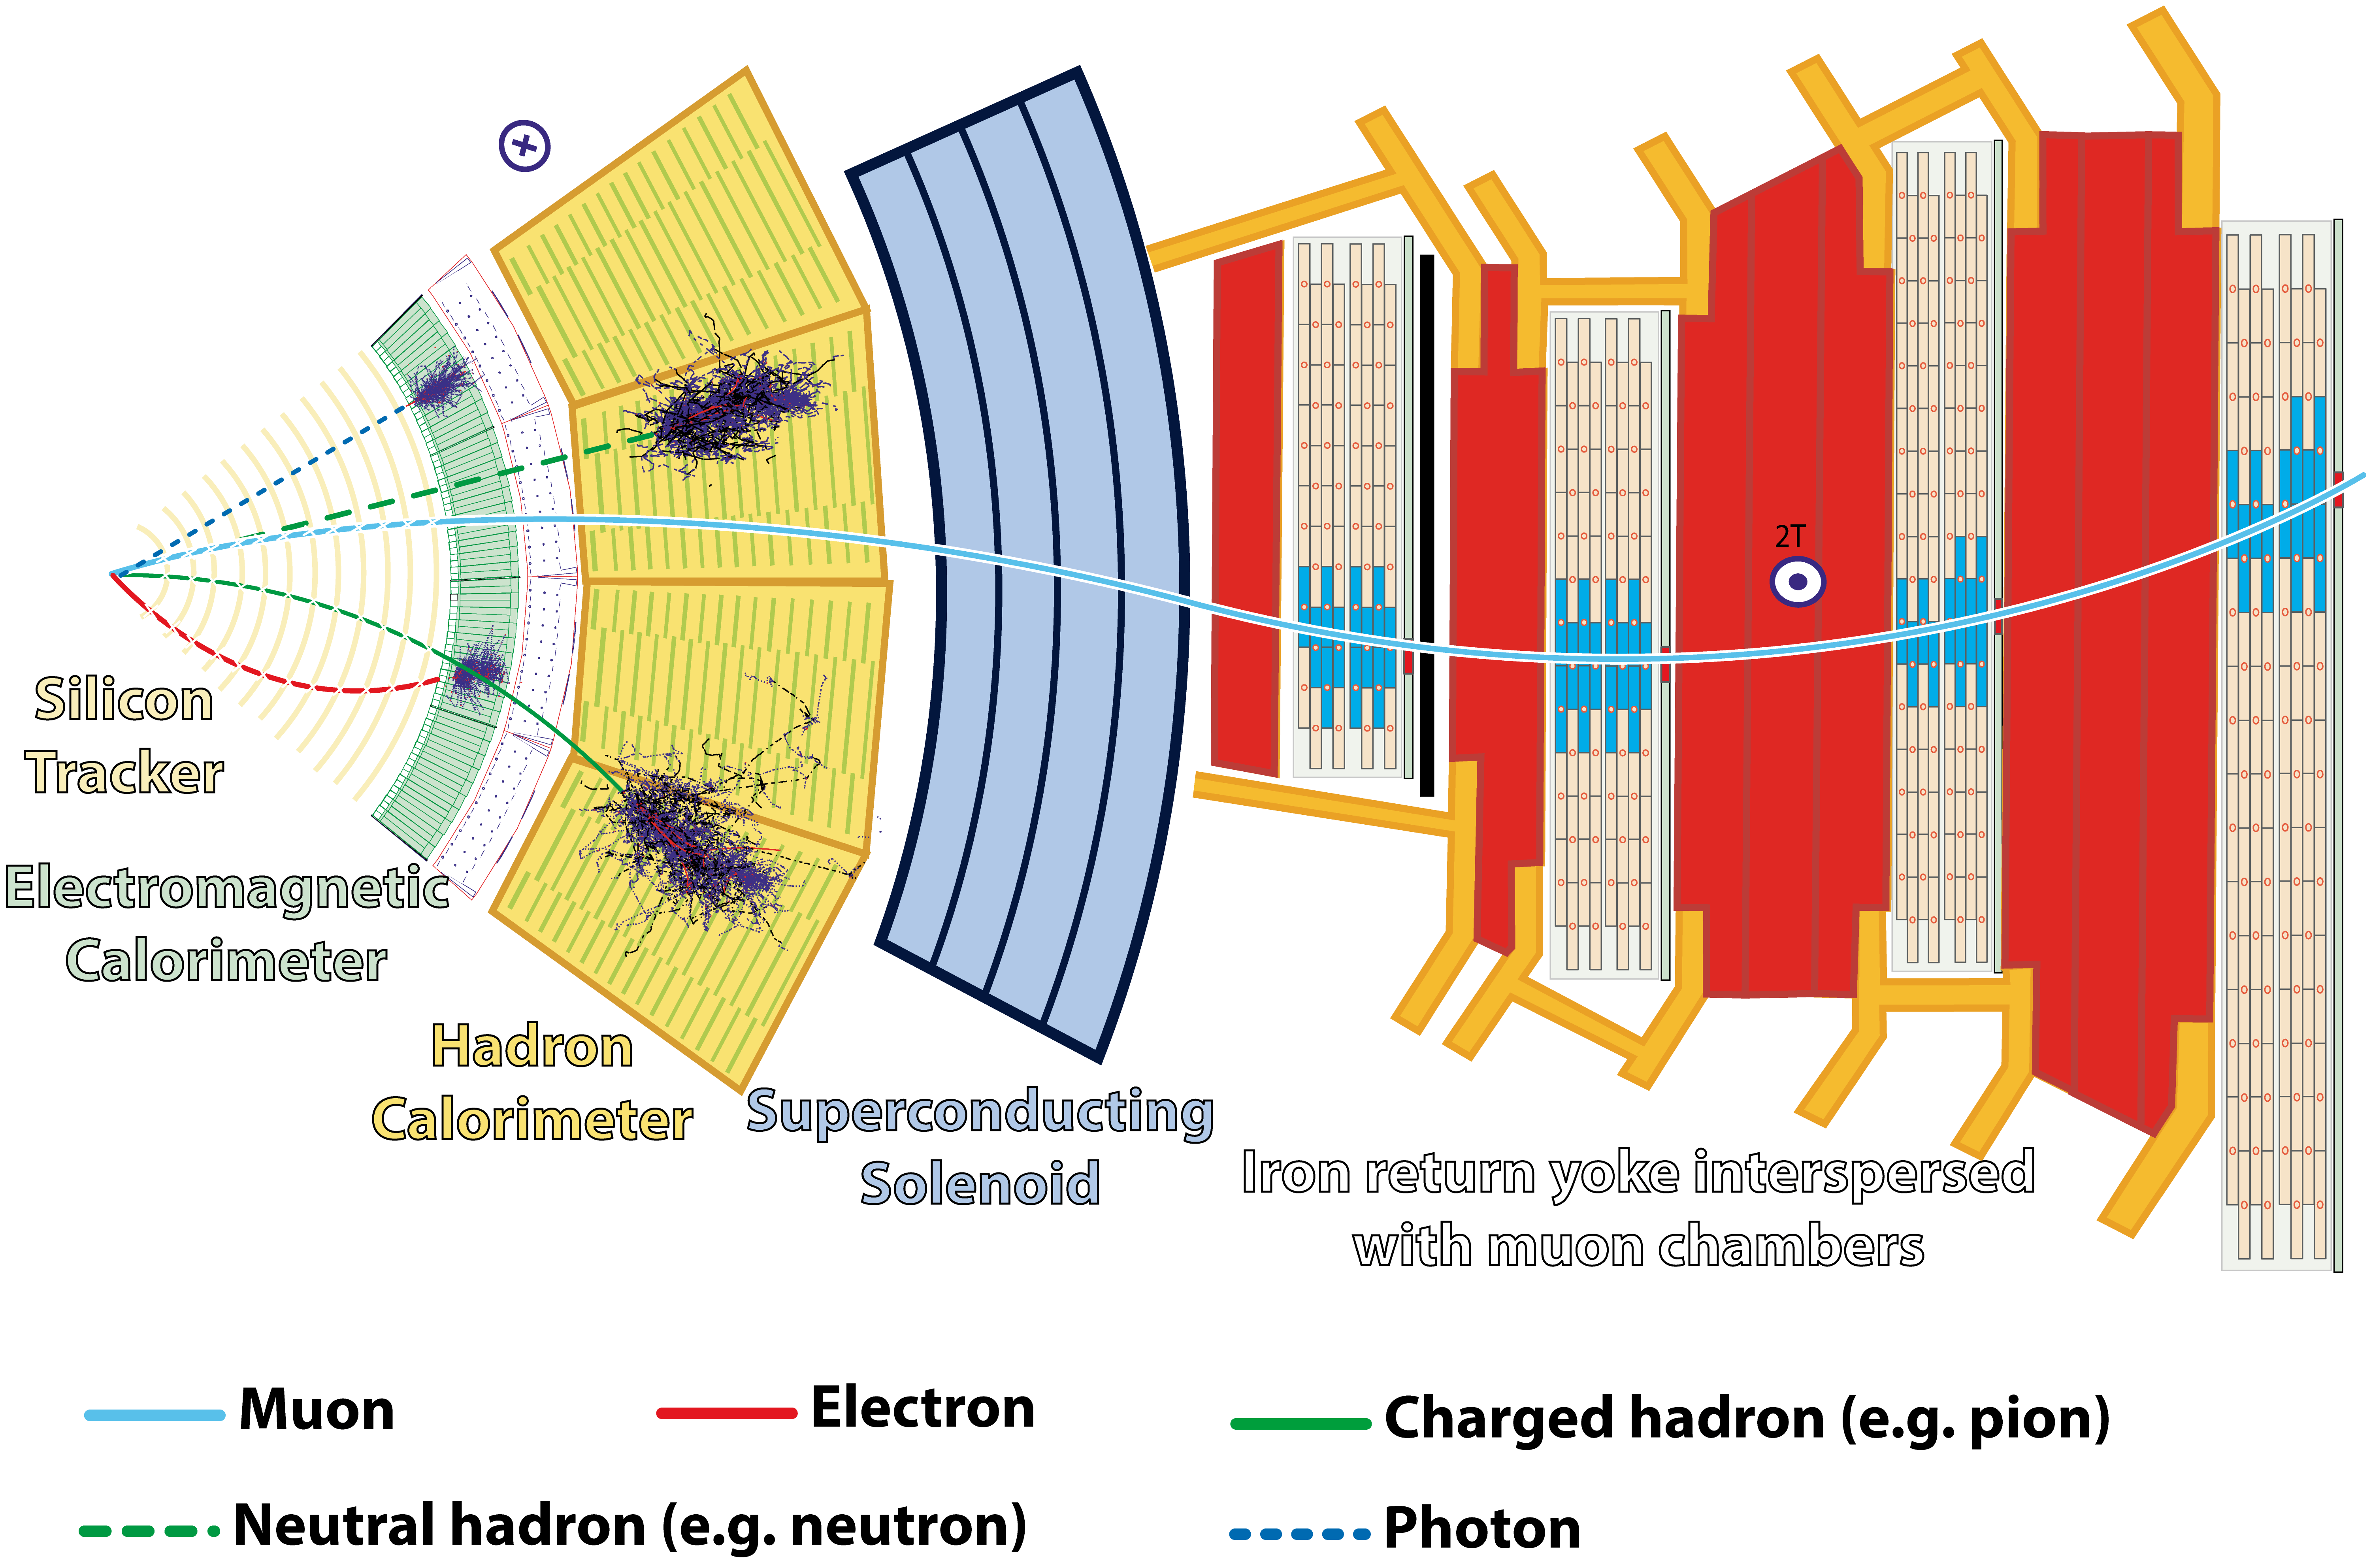
\includegraphics[width = \textwidth]{images/cms.png}
    \caption{Schematic structure of the CMS experiment}
    \label{cms}
\end{figure}
\subsection{Tracker}
Starting from the interaction point, the particles go through the tracker. This section is designed to have precise measurements of the tracks of charged particles and the primary interaction vertices.\\
The tracks are bent using the homogeneous magnetic field of 3.8 T, and the actual revelation is made with the silicon pixel detector in the innermost section, and with silicon microstrip after; overall, the tracker has a diameter of 2.5 m.\\
Pixel detectors are used to ensure high granularity, due to the huge number of tracks present.
This part of the apparatus is the one that withstands the highest amount of radiation.\\
The acceptance of the tracker is of $|\eta|<2.5$.\\
In the forward regions, two disks are present, one at each end, to improve impact parameter measurements and provide points with sufficient resolution for reconstructing secondary vertices from decays of particles containing \emph{c} or \emph{b} quarks.
\subsection{Calorimeters}
Outside the tracker, the electromagnetic calorimeter (ECAL) and then the hadronic calorimeter (HCAL) are located.\\
Calorimeters are used to absorb and measure the energy of all incoming particles (except for neutrinos, which essentially don't interact). \\
When high-energy particles traverse a dense medium, they produce secondary particles with lower energies due to the phenomenon called particle showering. The characteristics of these showers depend on the type of particle.\\
\textit{Electromagnetic showers} are produced by particles that interact mainly electromagnetically, such as electrons, positrons, and photons. Their length is related to the radiation length $X_0$ \footnote{Radiation length: mean length inside the material at which the energy of an electron is reduced due to bremsstrahlung by a factor $e^{-1}$; it's characteristic of a material.} of the material with the following formula:
\begin{equation}
    X = X_0 \frac{\ln(E_0/E_c)}{\ln 2},    
\end{equation}
where $E_0$ is the initial energy of the particle and $E_c$ is the critical energy \footnote{Critical energy: energy at which the bremsstrahlung rate coincides with the collision loss rate (for ionization and excitation)}.
So, to completely absorb the energy from the incoming particles, the calorimeters are designed to have a width equal to 2–3 times $X_0$. %numeri che vanno ricontrollati\\
\textit{Hadronic showers} are produced by particles that interact mostly strongly because of processes like hadron production, nuclear deexcitation and pion decay. This type of shower takes longer to develop, and its length scales with the nuclear interaction length:
\begin{equation}
    \lambda = \frac{A}{N_A \sigma_{abs}},
\end{equation}
where A is the mass number, $N_A$ is the Avogadro number and $\sigma_{abs}$ is the absorption cross-section.
\\
As a trivial example, we report the radiation length and interaction length for different materials in table \ref{x_0}.
\begin{table}[h]
\centering
    \begin{tabular}{c|c|c}
 Elements &$X_0 [g cm^{-2}]$ & $\lambda [g cm^{-2}]$ \\\hline
     H$_2$ &  61.28 & 50.8 \\\hline
     Si & 21.82 & 106.0\\\hline
     Fe & 13.84 & 131.9\\\hline
     Pb & 6.37 & 194 \\
    \end{tabular}
    \caption{Summary of radiation length and interaction length for some elements}
    \label{x_0}
\end{table}

Calorimeters need to be as precise as possible to detect the presence of missing energy, that is, the energy carried by particles that don't interact with the medium, like neutrinos or BSM particles, and that appear as energy that disappears during the event.
\subsubsection{ECAL}
The ECAL is a hermetic homogenous \footnote{homogenous vs sample tbw} calorimeter made of lead tungstate crystals (PbWO$_4$); it is used to measure the energy of the electromagnetic showers with the use of photodiodes and phototriodes.\\
Two parts of the ECAL can be distinguished: the barrel section, with pseudorapidity coverage of up to $|\eta|= 1.48$, and the endcaps, which extend the coverage up to $|\eta| = 3.0$.
The use of PbWO$_4$ is innovative, and it leads to the possibility of having a fast calorimeter due to the short scintillation decay time\footnote{Scintillation decay time: time required for scintillation emission light to decrease to $e^{-1}$ of its maximum} and with fine granularity, thanks to their high density and short radiation length ($X_0$ = 0.89 cm), which is important for the energy resolutions.\\
One of the driving criteria was to be able to detect the $H\longrightarrow\gamma\gamma$ decay.\\
To have further spatial precision, the endcaps also have a preshower detector within the region $1.653 < |\eta|< 2.6$, which is used to discriminate between a highly energetic photon and a pair of low-energy photons coming from the decay of short-lived particles like neutral pions. The preshower detector is made of a layer of lead and then of silicon; when a photon passes through, it makes an electromagnetic shower that is detected by the silicon sensors, and from which the energy of the photon is measured, leading to the discrimination.\\
Fig. \ref{ecal} shows a schematic representation of the ECAL.
\begin{figure}[h]
    \centering
    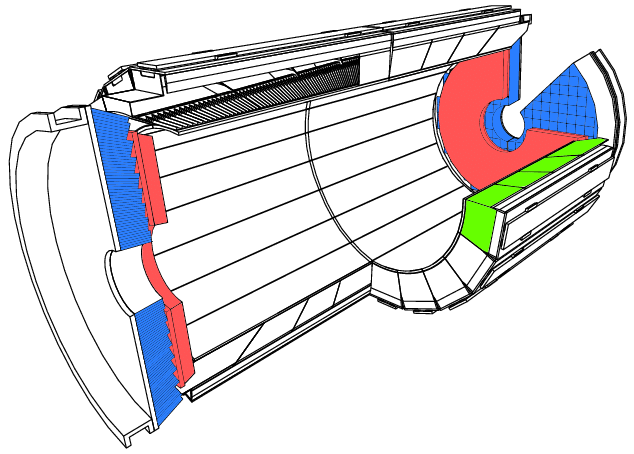
\includegraphics[width = 0.6\textwidth]{images/ecal.png}
    \caption{Schematic representation of the ECAL. In green the barrel, in blue the endcaps and in red the preshowers.}
    \label{ecal}
\end{figure}
\subsubsection{HCAL}
HCAL is a sampling calorimeter: there is an absorber made of steel and brass ($\lambda = 16.42 cm $) that slows the particles down, and plastic scintillators (with thickness that goes from 40 up to 75 mm) that measure the energy of the hadronic showers.\\
To guarantee the maximum pseudorapidity coverage, HCAL is composed of four parts:
\begin{itemize}
    \item the barrel (HB): it covers up to $|\eta| 1.3$, and its coverage in interaction lengths goes from 5.82$\lambda$ up to  10.6 $\lambda$, to which it must be added 1.1 $\lambda$ given by the ECAL.
    \item the endcap (HE): it covers the region 1.3 $<|\eta| < 3$ and contains about 34\% of the particles produced in the final state. This means that the HE needs high radiation tolerance, especially for $\eta\approx$3. Its coverage in interaction lengths is about 10$\lambda$.
    \item the outer calorimeter (HO): it's located outside the solenoid that surrounds HB, and it covers the central region in pseudorapidity (so up to $|\eta| 1.3$) to provide better containment for hadron showers, in particular late starting showers. It extends the coverage in interaction lengths of the HB to at least 11.8 $\lambda$.
    \item the Forward calorimeter (HF): it covers the region of highest pseudorapidity, where the particle fluxes are highest. This means the HF will need to be highly radiation resistant, which is why quartz fibres were chosen as active medium. However, because it exploits Cherenkov radiation for detection, it's mostly sensitive to electromagnetic showers, while it is practically insensitive to neutrons.
\end{itemize}

Fig. \ref{hcal} summarises the various components of HCAL.
\begin{figure}[ht]
    \centering
    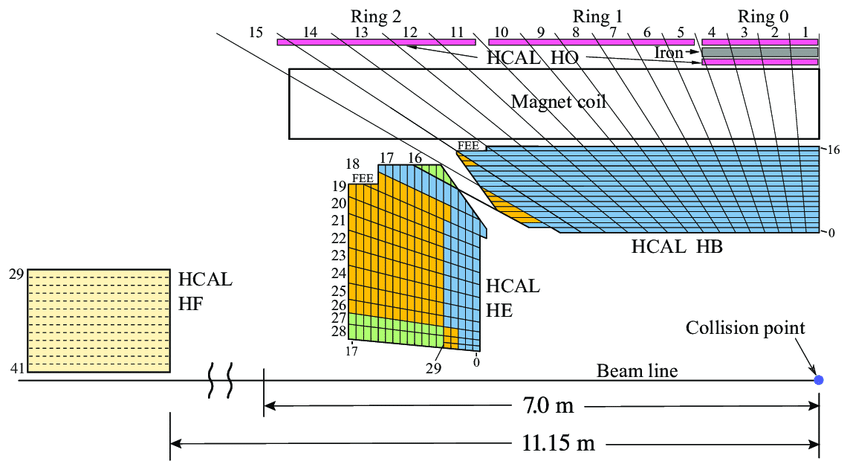
\includegraphics[width = 0.8\linewidth]{images/hcal.png}
    \caption{Schematic representation of a quarter of HCAL}
    \label{hcal}
\end{figure}
\subsection{Muon system}
Muons are a very useful tool that can be used to recognize signatures of interesting processes above the high background rate present. An example of process would be the decay $H\rightarrow ZZ\rightarrow 4 l$, where the two Z decay into charged leptons (the \textit{golden channel}). The case where the leptons are muons is the cleanest one, because the electrons interact with matter inside the detector, while muons are not affected as much.\\
The muon system has three functions: muon identification, momentum measurement, and triggering. \\
It is located inside the returning yoke of the magnetic solenoid, which is used as a hadron absorber as well as to bend the muons and study the momentum from its tracks; between the plates of the yoke, the particle detectors are set.\\
In the barrel region, the muon rate is small, as well as the background, and the magnetic field is uniform and contained in the yoke. So, in the region with $|\eta|< 1.2$ 250 drift tubes are used, and their arrangement provides a way to measure the muon time with good time resolutions.\\
In the endcap regions, the muon rate and the background are much higher, and the magnetic field is non-uniform, so for the region $0.9<|\eta|<2.4$ 540 cathode strip chambers are used instead.\\
A crucial characteristic of both the drift tubes and the cathode strip chambers is that they can each trigger on the muon $p_T$ with good efficiency and high background rejection, independently of the rest of the detector. However, because of the uncertainty, a complementary trigger system was added both in the barrel and endcap regions, consisting of resistive plate chambers that cover up to $|\eta|<1.6$.
Fig. \ref{muon_system} shows a schematic view of the muon system, with the various detection stations located between the yoke plates.
\begin{figure}[ht]
    \centering
    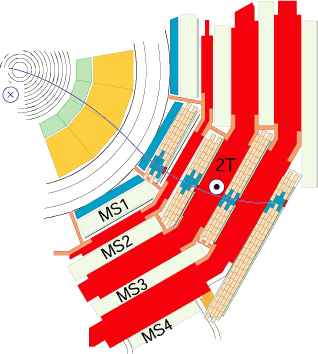
\includegraphics[width = 0.5\linewidth]{images/MuStations.png}
    \caption{Schematic focus representation of the muon system}
    \label{muon_system}
\end{figure}
\subsection{Trigger}
As we previously said, in LHC the beams in the proton interactions cross every 25 ns, and this brings a crossing frequency of 40 MHz. We also stated that multiple interactions happen at the same time.\\
However, the CMS experiment can record only about a thousand events per second.\\
This shows that a severe rate reduction has to take place to store and process data. This is made by the trigger system in two steps, where potentially interesting events are selected and stored for analysis.\\
The \emph{Level-1 trigger} (L1)  brings the rate from 40 MHz to 100 kHz in about 3.8 $\mu$s. It consists of custom-designed electronics that evaluate information from the detector (transverse energies from ECAL and HCAL, tracks isolation, muon trigger), reconstruct some information about the event (like the total transverse energy and the missing energy) and about the particles ($p_T$, $\phi \text{and} \eta$ coordinates), and decide if the event is to be kept or rejected based on the number of jets, thresholds on $p_T$ or $E_T$, and also the topology of the event.\\
The \emph{High Level Trigger} (HLT) brings the rate from 100 kHz to 1 kHz in about 300 ms. It is a software system implemented in a filter farm of about 30,000 commercial cores that further reconstructs the event and looks for more specific event signatures to decide whether to store an event. Because of the time requirements for this analysis, the events are reconstructed in multiple steps and rejected as soon as there is enough information to do so.
\section{Events Reconstruction}
As we introduced, particles of an event are detected by studying the hits left in the different sections of the detector. In principle, one would need only information from the specific subdetector, for example:
\begin{itemize}
    \item jets come from hadrons and photons, and their energy can be reconstructed inclusively without separating individual jet particles. This means that jet reconstruction can be done with the use of HCAL (and ECAL) only, without using information from muon detectors and trackers;
    \item missing transverse momentum and missing transverse energy can be reconstructed with the use of calorimeters only;
    \item isolated photons and electrons need information from ECAL only for reconstruction;
    \item tagging specific particles like $\tau$ leptons and b quarks that have hadronized can be done with information from tracker only;
    \item muons can be identified with information from the muon detectors only.
\end{itemize}
However, a more refined approach, called particle-flow (PF) reconstruction, allows a significant improvement in the description of an event. A brief summary of this approach follows, while a more comprehensive description can be found at Ref. \cite{particle_flow}.\\
In the PF approach, the basic elements from all subdetectors are used to identify each particle in the final state.
\subsubsection{Charged-particle tracks and vertices}
The first important element is the track reconstruction. For this, a combinatorial track finder based on Kalman Filtering (cit) is used to reconstruct the charged-particle trajectory and its properties: transverse momentum, origin, and direction. A track is accepted if it has at least a number of hits inside the tracker, and if it originates within a cylinder of a few mm of radius centred around the beam axis. 
\section{HL-LHC Upgrade}
\label{sec:HL-LHC}
To extend the sensitivity for new physics searches, a major upgrade of the LHC was decided, called the High Luminosity LHC (HL-LHC). With this upgrade, the luminosity of the collider will be greatly enhanced. \\
For this reason, a Long Shutdown (LS3) was planned for 2023. However, because of the COVID-19 pandemic, the LHC was forcefully shut down, and LS3 was postponed to the end of 2024, as can be seen from the schedule in fig. \ref{lhc_schedule}.
\begin{figure}
    \centering
    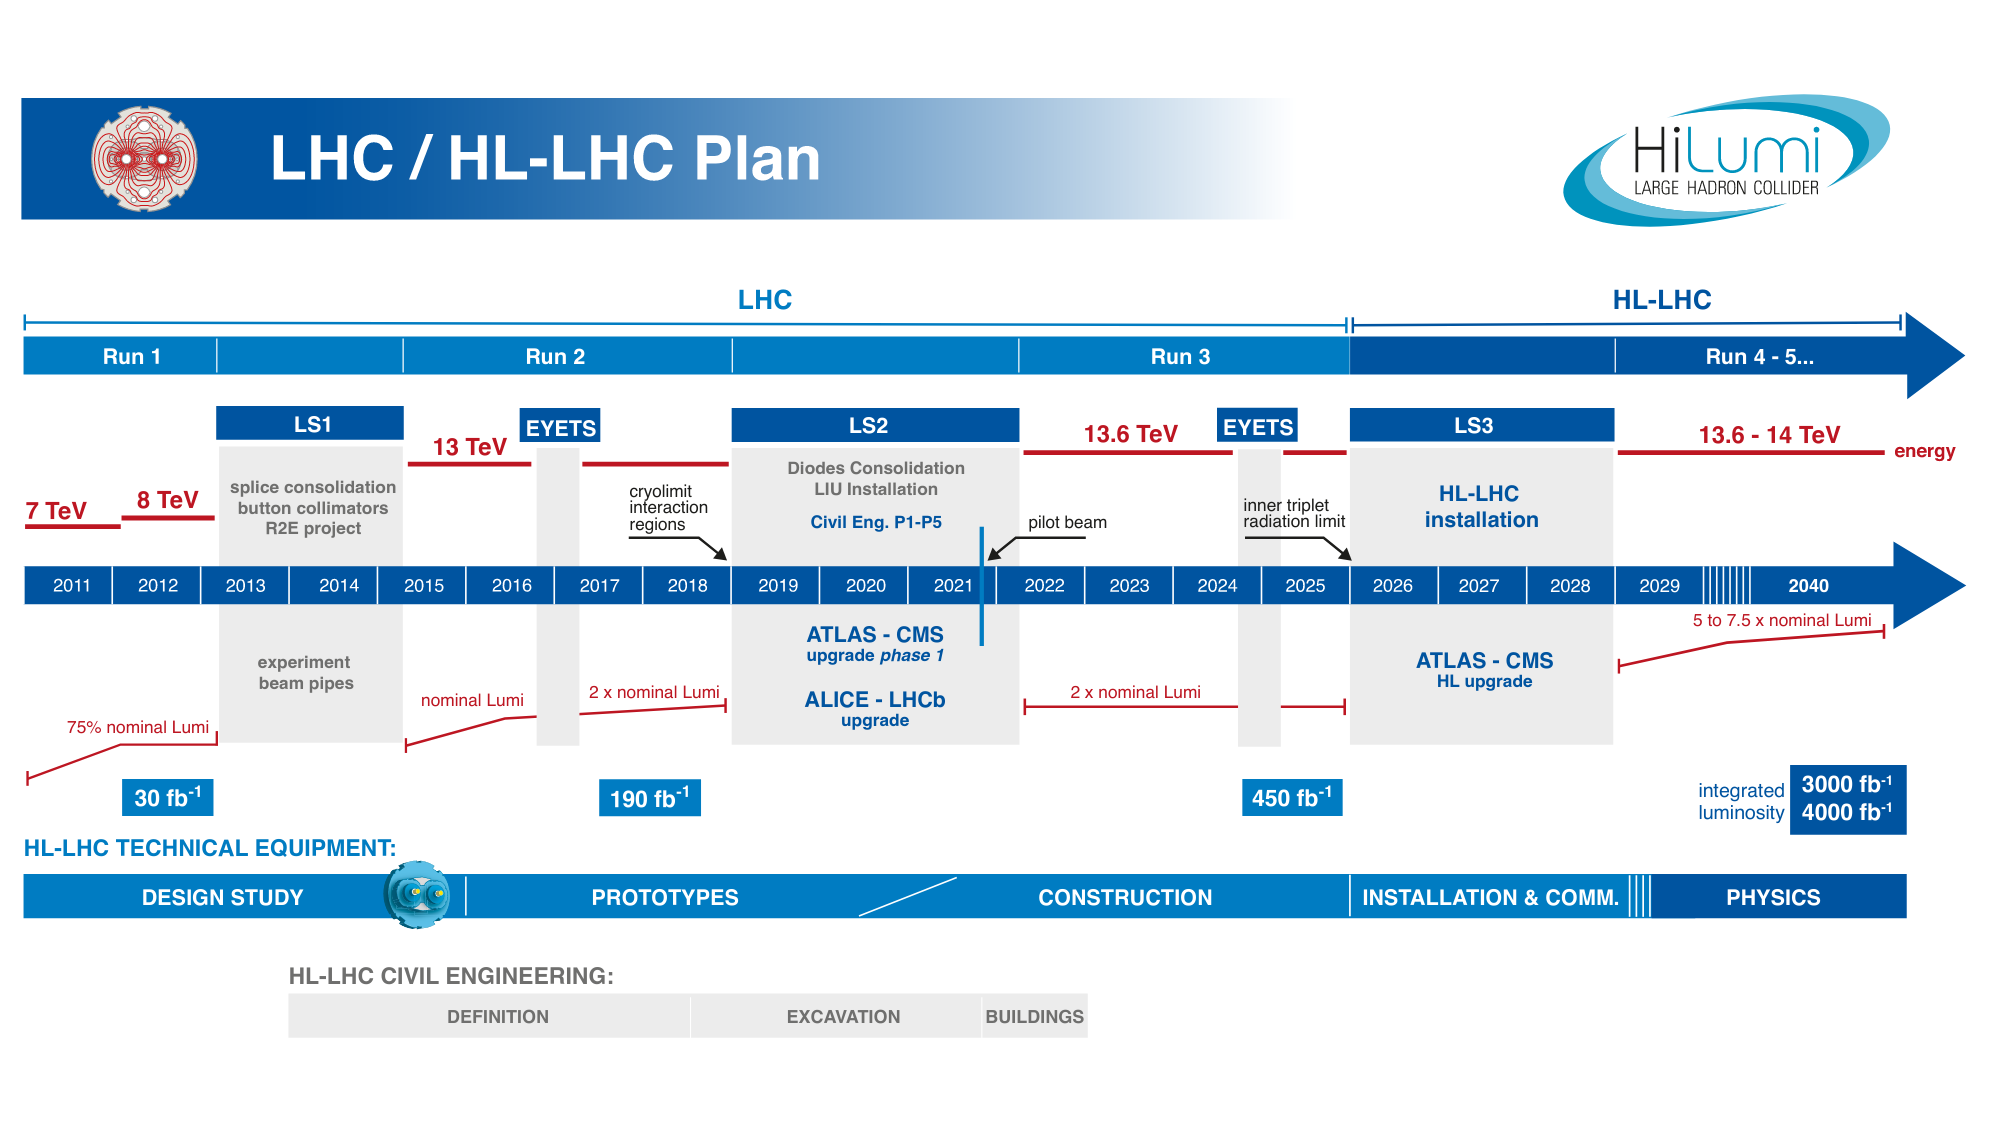
\includegraphics[width = \linewidth]{images/lhc_schedule.png}
    \caption{LHC Schedule considering the forced shutdown due to COVID-19}
    \label{lhc_schedule}
\end{figure}
Fig. \ref{hl_lumi} shows the peak luminosity and the integrated luminosity throughout the years and the expected values for the HL-LHC era.
\begin{figure}
    \centering
    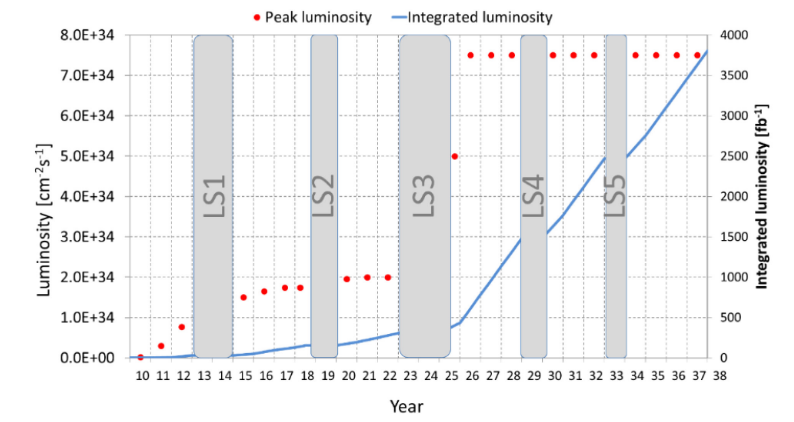
\includegraphics[width = \linewidth]{images/hl_lumi.png}
    \caption{Peak luminosity (red dots) and integrated luminosity (blue line) with the projection of performance of the HL-LHC phase after LS3.}
    \label{hl_lumi}
\end{figure}
The ultimate targets of the project are the following:
\begin{itemize}
    \item Peak luminosity of 7.5 x 10$^{34}cm^{-2}s^{-1}$;
    \item Integrated luminosity of 300-400 fb$^{-1}$ per year, with the goal of 4000 fb$^{-1}$ in the 12 years after the upgrade.
\end{itemize}
These targets require the main experiments ATLAS and CMS to cope with an average pile-up of at least 140, which should increase to 200 in the later period, and obviously increased radiation.
For these reasons, the main equipment modifications will be done in the two major experiment locations, LHC Point 1 (P1 - ATLAS) and LHC Point 5 (P5 - CMS).\\
\subsection{Upgrades to the experiment}
Some of the most relevant upgrades to the CMS detector are listed. The complete upgrade project is reported in Ref. \cite{phase2_tdr}.\\
\begin{itemize}
    \item The silicon tracker must be replaced because of the radiation damage it will sustain by the end of Run3. Furthermore, to maintain the resolution of track reconstruction at high pileup, the granularity of both the inner pixel tracker and the outer tracker needs to be increased. This will improve the $p_T$ resolution, decreasing the trigger rate at a given transverse momentum.
    \item To have a more efficient trigger at low $p_T$ (in particular for $p_T\geq 2$GeV), a new approach will be adopted, that is, the addition of tracking information at L1. This leads to the necessity of new hardware to incorporate the tracking information. 
    \item The endcap calorimeters will also suffer significant radiation damage. The replacement planned is called High Granularity Calorimeter (HGCAL), and will have both the electromagnetic and the hadronic sections. It will consist of a sampling calorimeter with silicon detectors in the inner region, and scintillators in the outer region. Given the granularity of HGCAL, it will also be able to identify tracks and discriminate between charged pions and muons, which, as stated, are present in the forward region. The electromagnetic section will consist of tungsten and copper plates interleaved with silicon scintillators; its width will be 25$X_0$ and 1 $\lambda$. The hadronic section will have a front section of bass and copper plates interleaved with silicon sensors for a width of 3.5$\lambda$, and a "backing hadron calorimeter" similar to HE, with brass plates interleaved with plastic scintillating tiles to provide an overall depth of $\approx10\lambda$ for the full calorimeter.
    \item For CMS in particular, it is of vital importance to improve the resolution of muon detection, especially in the forward region, and this will be done by adding muon chambers and muon detectors, so that a more precise measurement of $p_T$ at L1 level will keep a manageable trigger rate without having to increase the threshold, and so risking to potentially lose new physics at low $p_T$.
    \item Furthermore, Phase-2 will see extended coverage of the inner tracker up to $|\eta|=4$, and this upgrade must be matched with an extension of the muon detection system in the very forward region as well, because the tracker alone cannot identify muons. For this reason, the muon system will be expanded up to $|\eta| \approx 3$. The increase in acceptance in this region is very useful, for example in studying multi-lepton final states like the golden channel.
    \item Latency for L1 was limited to 3.4 $\mu$s by the tracker readout. In Phase-2, it will be increased to 12.5 $\mu$s to provide sufficient time for the hardware track reconstruction and the matching of tracks from the muon system and the calorimeters. With the upgrades, the trigger acceptance rate will be 500 kHz for a PU of 140.
\end{itemize}
\subsection{Physics program}
Thanks to the upgrade, the available dataset after the end of the HL-LHC era will be ten times larger than the one available now. This means that processes with very low cross-section and/or decay branching fractions might be visible.\\
Starting with the Higgs boson, HL-LHC will permit the measurement of the Higgs trilinear self-coupling, and subsequently the study of the Higgs potential. Furthermore, a more detailed study of the properties of the Higgs boson will be possible, for example, the CP, the total width, and the measurement of very rare decay channels.\\
HL-LHC will also allow the search for a more extended Higgs sector, both at higher and lower masses than 125 GeV.\\
All the preliminary studies of the detector performance are made using the Delphes fast simulation \cite{delphes}.\\
A list of some of the objectives for the HL-LHC are reported \cite{HL-LHC_Higgs}, \cite{phase2_tdr}.
\subsubsection{H$\longrightarrow $ZZ$^* \longrightarrow 4 l$}
As previously stated, this is the golden channel in the study of the Higgs boson. Electrons and muons can be measured very accurately, with high efficiency and excellent energy and momentum resolution. This means that the final state can be reconstructed, and this leads to a signal with high purity, which is measured as a peak over a smooth background.\\
This channel is very interesting because studying the angular distributions, like the angle between the ZZ decay planes and the decay angles in these planes, allows a detailed analysis of the CP properties of the Higgs boson and of its total width.\\
The projections of Phase 2 show a significant increase in the selection efficiency after a full selection. 

\subsubsection{H $\bm{\longrightarrow \mu\mu}$}
So far, the only decay modes observed for the Higgs boson have been the ones to the third generation of fermions (\emph{t}, \emph{b}, $\tau$), and with the vector bosons. \\ 
So, an important test to the SM is the study of the Higgs coupling with the fermions of the second generation, which, however, have smaller values and smaller experimental rates.\\
The easier one from the experimental side is the decay of the Higgs boson in two muons, which has a branching fraction expected from the SM of $2.2 x 10^{-4}$. Furthermore, the events can be fully reconstructed, and the signal will appear as a small bump on the di-muon background from Drell-Yan events, and this means that an excellent resolution on the di-muon mass is needed.
\\
Evidence of the Higgs decay in a pair of muons was presented in 2020 with an observed (expected) significance of 3.0 (2.5) standard deviations \cite{H_mumu}.\\
The simulations made of the upgraded Phase-2 tracking detector show an improvement on the mass resolution of 40\%, and an improvement of 20\% on the reconstruction efficiency of the muon pair.
\subsubsection{H $\bm{\longrightarrow \tau \tau}$}
From projections, modifications of the Higgs coupling constant to tau leptons from its SM value can be measured with a precision of 2-5\%, and from BSM Higgs models, modifications comparable or larger to this are to be expected, especially in the hypothesis of multiple Higgs doublets.\\
This makes the H $\longrightarrow \tau \tau$ a good channel to search for new physics.\\
The study of this channel heavily relies on the performance of the whole CMS detector, because the analysis uses electrons, muons, hadronic taus, jets, and missing transverse energy; for this reason, high efficiency and low misidentifications are needed to control the high background. \\
\subsubsection{Higgs boson pair production}
One of the upgrade's main objectives is observing the trilinear coupling of the Higgs boson. This process is also sensitive to BSM physics, which might modify the rate of pair production. Various final states of the Higgs pair will be studied, with their branching fractions are reported in table \ref{pair production BR}:
\begin{itemize}
    \item $\bm{bb\gamma\gamma}$: the signal events contain two high-$p_T$ photons and two high-$p_T$ jets coming from b quarks. For this channel, only 320 events per experiment are expected to be produced with an integrated luminosity of 3 ab$^{-1}$, but it's one of the most sensitive channels to HH production. The background can be mainly divided into two categories: the resonant one and the non-resonant one. The resonant category contains processes like ZH, $t\Bar{t}H$, $b\Bar{b}H$, where the Higgs boson decays in two photons; the non-resonant category contains processes like $b\Bar{b}\gamma\gamma$, $jj\gamma\gamma$, where $j$ are jets from light quarks and are mis-tagged as b jets, or also processes like $b\Bar{b}jj$ or $b\Bar{b}j\gamma$, with one or two jets are misidentifies as photons. The non-resonant backgrounds have cross-sections several times larger than the resonant one, but they are expected to be suppressed by the low rates of misidentification and mis-tagging, also thanks to the improvement that will be obtained on both the parameters (cambiare la parola) during Phase-2.
    \item $\bm{bb\tau\tau}$: for an integrated luminosity of 3 ab$^{-1}$, about 9000 $bb\tau\tau$ events are expected. However, there is an overwhelming contribution of $t\Bar{t}$ background with fully leptonic decays, as well as Drell-Yan production of a Z boson decaying into a pair of tau leptons that are produced with jets coming from light quarks misidentified as b quarks, and single Higgs production, in particular ZH and $t\Bar{t}H$, while QCD multi-jet background is negligible in the signal region. The discrimination of the signal is challenging because of the incomplete reconstruction of the event due to the presence of missing energy from neutrinos of the $\tau$ decays. A cinematic bounding variable is introduced to better discriminate the $t\Bar{t}$ background from the di-Higgs signal. The expected significance for the production in this final state with the combination of $\tau_h \tau_h$ and $\tau_h \tau_{mu}$ is 0.9 standard deviations.\\
    The $\tau \tau$ final state is also interesting for testing BSM physics, for example introducing additional interactions between leptons and hadrons.
    \item $\bm{bbVV}$: both $bbWW$ and $bbZZ$ are considered, even though the most relevant in terms of statistics is the prior. During HL-LHC, about 1800 events are expected from the fully leptonic decay of the W bosons. The dominant background is given by $t\bar{t}$ production with fully leptonic decay. Selected events are required to have two b-tagged jets and two opposite-sign leptons. The results from the preliminary studies suggest a promising contribution of this final state when combined with the other final states that have been considered.
    For the $bbZZ$ decay, 17 events are expected, and they are required to have at least 4 muons or electrons, in addition to the two b-jets coming from the decay of one of the H bosons. The two Z boson candidates are formed from pairs of opposite-charge leptons, with invariant mass around the nominal Z mass; the most relevant background comes from single H production with 4$l$ in the final state.
    \item $\bm{bbbb}$ It has the largest branching fraction, with an expected number of events at the end of HL-LHC of about 37000. However, it is also the channel with the largest QCD multi-jet background. For this reason, the events from this channel are divided into two categories: 
    \begin{itemize}
        \item in the case where the four b-jets can be reconstructed separately the category is called "resolved", and multivariate methods are explored to face the overwhelming background; resolved topology corresponds to the large majority of SM events. In the analysis, the four selected b-jets are combined into two Higgs candidates, H$_1$ and H$_2$ so that the invariant mass is minimal. Because of the large QCD background, a multivariate variable is defined using a Boosted Decision Tree (BDT) to identify the HH signal contribution, and it is used as a discriminator variable
        \item in the case where the invariant mass of the HH system is big, it can happen that the two b-jets from the same H decay overlap and are reconstructed as a single, larger jet, and this category is called "boosted". Boosted topology helps the discrimination of the signal from the background, and provides sensitivity to BSM physics as well, in scenarios where the pair production is enhanced at high values of $m_{HH}$, for example with the presence of ttHH and ggHH contact interactions. Algorithms for b-tagging are used on the sub-jets contained inside the b-jets.
    \end{itemize}  
\end{itemize}
\begin{table}[ht]
    \centering
    \begin{tabular}{c|c}
        Channel & BR [\%] \\\hline 
        $bbbb$ & 33.9 \\\hline
        $bb\tau\tau$ & 7.3 \\\hline
        $bbVV$ (FL) & 1.73 \\\hline
        $bb\gamma\gamma$ & 0.26 \\\hline
    \end{tabular}
    \caption{Branching ratios for the dominant channels of pair production. For the gauge bosons, only the fully leptonic (FL) decay is considered}
    \label{pair production BR}
\end{table}

The different channels are combined statistically, assuming SM Higgs branching fractions. Assuming the presence of a SM signal, the total expected significance is 2.6 $\sigma$; on the contrary, in the background only hypothesis, the expected upper limit on the SM pair production cross-section can be set to 0.77 times the SM prediction.\\
Prospects for the study of the H self-coupling are studied. In the hypothesis of SM HH signal exists, the following confidence intervals can be set:
\begin{equation}
    \kappa_{\lambda} = [0.35, 1.9] \quad 68 \% \text{CL}
\end{equation}
\begin{equation}
    \kappa_{\lambda} = [-0.18, 3.6] \quad 95 \% \text{CL};
\end{equation}
in the hypothesis of background only, upper limits on the HH SM cross-section are derived as a function of $\kappa_{\lambda}$.\\
The results expected are reported in fig. \ref{prospect_HH}.

\begin{figure}
    \centering
    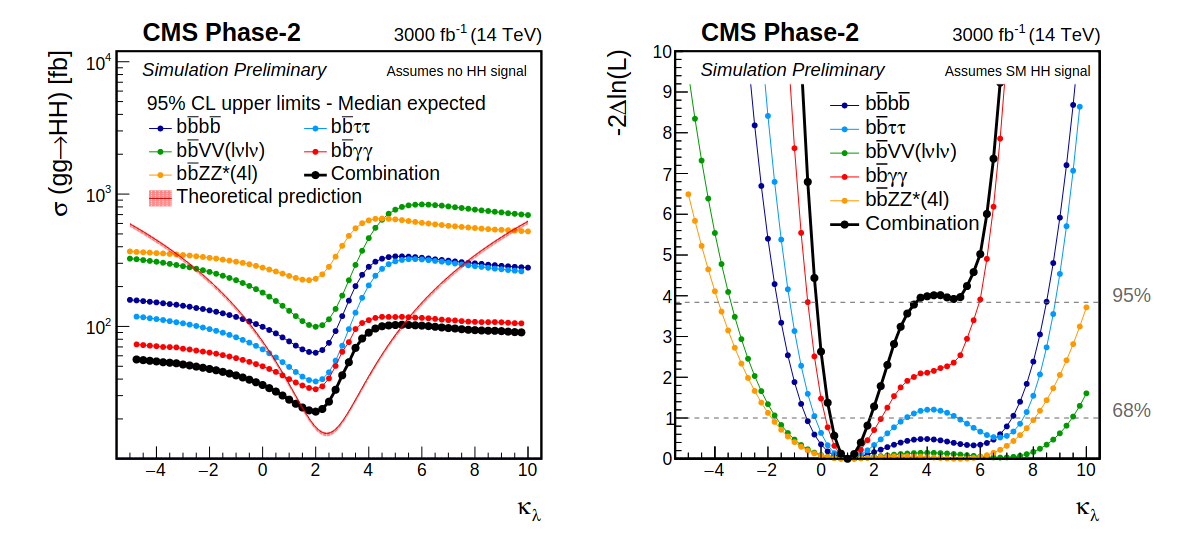
\includegraphics[width =\linewidth]{images/prospects_HH.png}
    \caption{Left: upper limit at 95\% CL on the HH production cross-section as a function of $\kappa_{\lambda}$; the red line shows the theoretical production cross-section. Right: expected likelihood scan as a function of $\kappa_{\lambda}$}
    \label{prospect_HH}
\end{figure}
\subsubsection{Vector Boson Scattering}
Vector Boson Scattering (VBS) is a powerful tool for investigating new physics, because of the high sensitivity to the electroweak symmetry breaking.\\
In particular, the Higgs field not only gives mass to the vector bosons, but also unitarizes the scattering amplitudes of longitudinally polarized bosons, by providing them with the longitudinal degrees of freedom needed to prevent the theory from diverging at high energies.\\
If SM is an effective theory with an additionally strongly-coupled sector, the unitarization of the VBS wouldn't come from the Higgs boson only, but from this new sector as well, which would appear at high energy scales.\\
For this reason, the observation of VBS would help in probing these scales.\\
At HL-LHC the VBS will be accessible when two quarks from the beam protons emit vector bosons, which then interact with each other. The two quarks deflecting will create jets that can be tagged to identify this category of events.\\ 
An example of event is shown in fig. \ref{vbs}
\begin{figure}[ht]
    \centering
    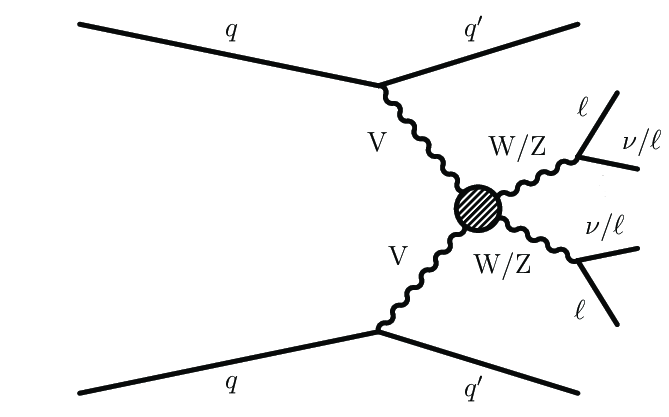
\includegraphics[width=0.4\linewidth]{images/vbs.png}
    \caption{Feynman diagram that shows an example of VBS with fully leptonic final state}
    \label{vbs}
\end{figure}
However, this category of events has a small cross section and suffers from the presence of a very high irreducible background, that is, the production of vector bosons and hadronic jets via strong interactions, to which the misidentification of jets-leptons has to be added.\\
For these reasons, the improvements from the upgrade will be beneficial, in particular the improvement on the jet-lepton misidentification, the extension in coverage of the tracking system up to $|\eta| = 4$ and the highly granular forward calorimeter, which will help with the contamination from jets coming from pileup.

\subsubsection{Other searches}
Studies on B physics are expected to be feasible, in particular in the case of rare processes like $B^0_{(s)}\longrightarrow \mu^+ \mu^-$ decays.\\
Furthermore, other sectors of SM and BSM are expected to be probed, for example, further studies on particles predicted from the SUSY framework, exotica searches, such as different SM extensions, dark matter, and new particles related to mechanisms that might give mass to the light neutrinos.\\


\chapter{The Flashsim framework}
\label{chap:chapter_4}
Flashsim is an innovative framework created in Pisa as a solution for the problem of simulations in High Energy Physics.

It exploits the flexibility of deep learning to skip the most computationally expensive steps of Monte Carlo simulations.

\section{Machine Learning}

Dummy text.

\subsection{Example Subsection}

Dummy text.

\subsubsection{Example Subsubsection}

Dummy text.

\paragraph{Example Paragraph}

Dummy text.

\subparagraph{Example Subparagraph}

Dummy text.

\chapter{Data Analysis}
\label{chap:chapter_5}


Dummy text.

\section{Example Section}

Dummy text.

\subsection{Example Subsection}

Dummy text.

\subsubsection{Example Subsubsection}

Dummy text.

\paragraph{Example Paragraph}

Dummy text.

\subparagraph{Example Subparagraph}

Dummy text.

\chapter{Results}
\label{chap:chapter_6}


Dummy text.

\section{Example Section}

Dummy text.

\subsection{Example Subsection}

Dummy text.

\subsubsection{Example Subsubsection}

Dummy text.

\paragraph{Example Paragraph}

Dummy text.

\subparagraph{Example Subparagraph}

Dummy text.


% \backmatter  % Template v2 fixes: this just breaks things

% Template v2 fixes: Bibliography belongs before appendix
\printbibliography
\appendix
\chapter{Symmetry breaking for Abelian Gauge Theory}
In this chapter, we briefly explain the behavior of gauge theories under symmetry breaking. \\


So, let us first consider a Lagrangian with the form:

\begin{equation}
    \mathcal{L} = \partial_{\mu}\phi^{\dagger}\partial^{\mu}\phi - \mu^2\left(\phi^{\dagger} \phi\right) - \lambda \left(\phi^ {\dagger}\phi\right)^2
\end{equation}
So there is gauge symmetry, but there's not a gauge field.\\
If $\mu^2<0$ the field has its minimum in:
\begin{equation}
    \langle \phi \rangle_0 \equiv v = \sqrt{\frac{\mu^2}{\lambda}}
\end{equation}



We can parametrize $\phi$ with a field that describes the fluctuations around the minimum:
\begin{equation}
    \phi(x) = \left(v + \eta(x)\right)e^{i \theta(x)}
\end{equation}
where $\theta(x)$ takes into account the gauge symmetry.\\
Substituting into the Lagrangian:
\begin{equation}
    \mathcal{L}=\partial_{\mu}\eta\partial^{\mu}\eta - 4 \lambda v^2 \eta^2 + v^2 \partial_{\mu}\theta\partial^{\mu}\theta + O(\eta^3)
\end{equation}
So, like in the global case, we find two particles, one massive, $eta$, and one massless, $\theta$, that is associated with the gauge symmetry, so it is a gauge boson.\\
Let us now consider a Lagrangian with the form:
\begin{equation}
    \mathcal{L} = \left(D_{\mu}\phi^{\dagger}\right) \left(D^{\mu} \phi\right) - \mu^2\left(\phi^{\dagger} \phi\right) - \lambda \left(\phi^ {\dagger}\phi\right)^2 - \frac{1}{4} F_{\mu\nu}F^{\mu\nu},
\end{equation}
where $D_{\mu}= \partial_{\mu} + i e A_{\mu}$ is the covariant derivative of the interaction field and keeps the field invariant under gauge transformations.
This Lagrangian is invariant under any local transformation from the $U(1)$ group.\\
If we consider the case $\lambda >0, \mu^2<0$ we obtain:
\begin{equation}
    \begin{cases}
        \langle\phi\rangle_0 \equiv \frac{v}{\sqrt{2}} = \sqrt{\frac{\mu^2}{2\lambda}}\\
        \langle A_{\mu} \rangle_0 = 0
    \end{cases}
\end{equation}
We can parametrize the field in this case as well:
\begin{equation}
    \phi(x) = \left(v + \eta(x)\right)e^{i \theta(x)}
\end{equation}
If we now consider the gauge transformations both for the field and the interaction field:
\begin{equation}
    \begin{cases}
        \phi(x)\rightarrow e^{-i\Lambda(x)}\\
        A_{\mu}(x)\rightarrow A_{\mu}(x) - \frac{1}{\alpha}\partial_{\mu}\Lambda(x)
    \end{cases}
\end{equation}
and we fix the gauge, that is, we decide the ambiguity on the gauge transformation that leaves the system invariant, by choosing for example:
\begin{equation*}
    \Lambda(x) = \theta(x)
\end{equation*}

we find that the reparametrized field now has a simpler form:
\begin{equation}
    \phi(x) = \eta(x) + v
\end{equation}

Inserting in the Lagrangian we find:
\begin{equation}
      \mathcal{L}= - \frac{1}{4} F_{\mu\nu}F^{\mu\nu} + \alpha^2 v^2A_{\mu}A^{\mu} + \partial_{\mu}\eta\partial^{\mu}\eta - 4 \lambda v^2 \eta^2 + O(\eta^3)
\end{equation}

So, we can see that, if the Lagrangian has a gauge symmetry, and we add a mechanism of spontaneous symmetry breaking, the Lagrangian keeps its gauge symmetry (we can still apply the transformations previously defined without changing the Lagrangian), but we also obtain a new particle, $\eta$, massive, and the gauge field as well obtains mass.\\
This mechanism is called Abelian Higgs mechanism.\\
The physical case uses a non-Abelian group, and in this way it theorizes four gauge bosons.

\chapter{Summary of the properties of elementary particles}
\label{app_particles}
A summary of the most important characteristics of SM elementary particles is reported.
\section{Leptonic sector}
\begin{table}[hb]
    \centering
    \begin{tabular}{c|c|c|c}
         Particle & mass [MeV]& Q & Y \\ \hline
         $e$ & 0.511 & -1  & -2\\ \hline
         $\nu_e$& $<0.8 10^{-6}$& 0 & 0 \\\hline    
         $\mu$ & 105.6& -1 &-2 \\\hline
         $\nu_{\mu}$ & & 0  & 0\\\hline
         $\tau$ & 1776.86 & -1 & -2\\\hline
         $\nu_{\tau}$ & & 0 & 0\\\hline
         
        
    \end{tabular}
    \caption{Summary of the leptonic sector}
    \label{lepton_summary}
\end{table}
\section{Quark sector}
\begin{table}[hb]
    \centering
    \begin{tabular}{c|c|c|c}
         Particle & mass [MeV] & Q &  Y \\ \hline
         u & 0.511 & +2/3  & \\ \hline
         d & & -1/3 & \\\hline
         c & 0.511 & +2/3  & \\ \hline
         s & & -1/3 & \\\hline         
         t & 0.511 & +2/3  & \\ \hline
         b & & -1/3 & \\\hline
         
 
    \end{tabular}
    \caption{Summary of the quark sector}
    \label{quark_summary}
\end{table}
\section{Gauge bosons sector}
\begin{table}[hb]
    \centering
    \begin{tabular}{c|c|c|c|c}
         Particle & mass [GeV] & S & Q  & Y \\ \hline
         W & 80.3 &1& $\pm$1 & 0 \\ \hline
         Z & 91.19 & 1 & 0 & 0 \\\hline
         $\gamma$ & 0&1 & 0 &  0\\\hline
         $g$ & 0 & 1& 0 & 0 \\\hline
         H & 125.25 & 0 & 0 & 1 \\\hline 
 
    \end{tabular}
    \caption{Summary of the gauge boson sector}
    \label{gauge_summary}
\end{table}

\chapter{$\kappa$-framework and results}
\label{kappa_framework}
The $\kappa$-framework is one of the tests on the SM. It consists of letting the various coupling constants vary and then studying, using a maximum likelihood test, the most probable value for the coupling constant.\\
In particular, every coupling constant is multiplied by a scaling factor $\kappa$

%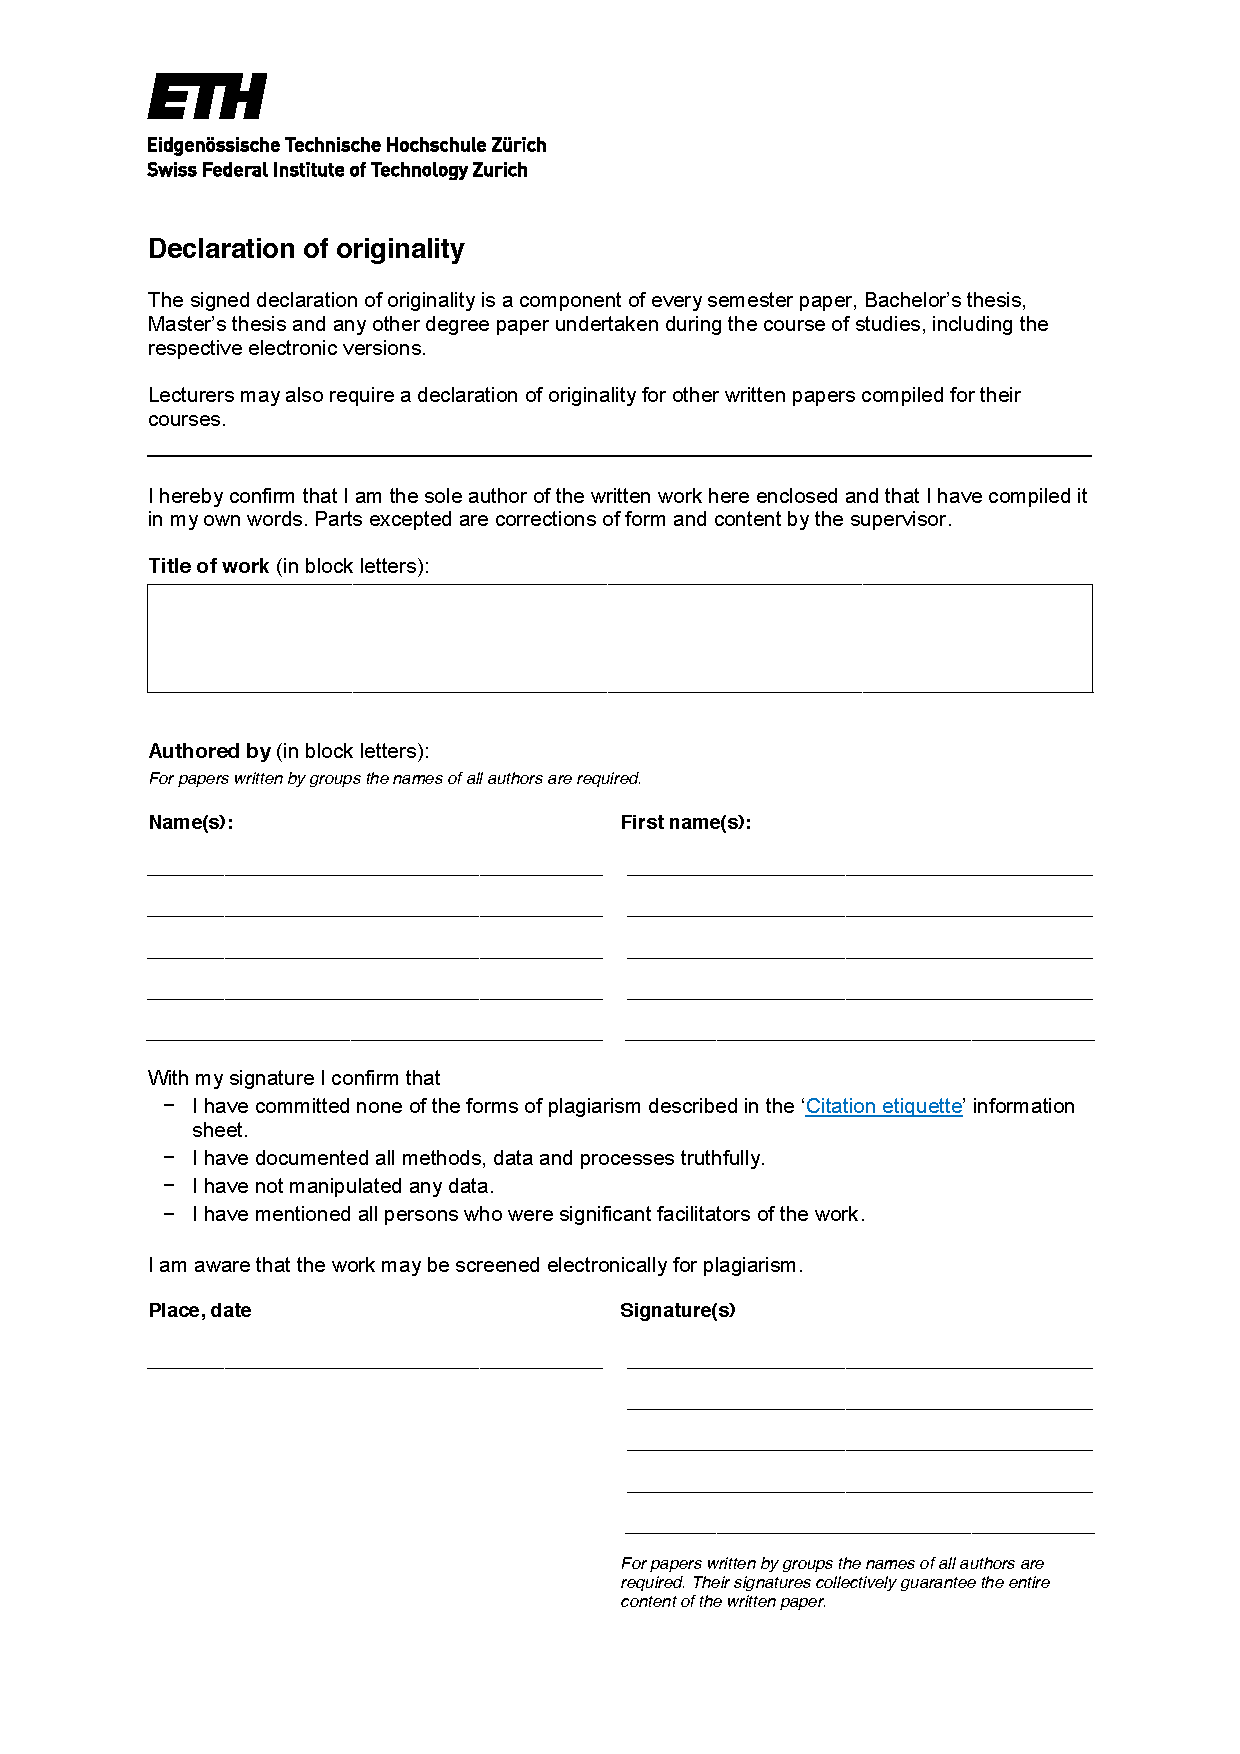
\includepdf[pages={-}]{eth-template/declaration-originality.pdf}

\end{document}
